\documentclass[a4paper,12pt,twoside]{report} % openright


\def\authorname{Douglas Boyle\xspace}
\def\authorcollege{Churchill College\xspace}
\def\dissertationtitle{Optimising compiler from OCaml to WebAssembly}


\def\wordcount{11977} %%% OVER LIMIT! MUST GET BELOW 12k


\usepackage{epsfig,parskip,setspace,tabularx,xspace}

\usepackage[pdfborder={0 0 0}]{hyperref}    % turns references into hyperlinks
\usepackage[margin=25mm]{geometry}  % adjusts page layout
\usepackage{graphicx}  % allows inclusion of PDF, PNG and JPG images
\usepackage{verbatim}
\usepackage{docmute}   % only needed to allow inclusion of proposal.tex
\usepackage{amsmath}
\usepackage{dirtree}

\usepackage{float}	

\usepackage{cprotect}

\usepackage{bytefield}
\usepackage{ebproof}
\usepackage{listings}
 \lstset{
  basicstyle=\ttfamily,
  mathescape
}

\pdfminorversion=7


\usepackage{epstopdf}
\epstopdfsetup{outdir=./}

\graphicspath{{figures/}}

\usepackage{fancyvrb}

%\includeonly{chapters/implementation}
%\includeonly{diss.bib}

\usepackage[backend=bibtex, sorting=none, urldate=iso8601]{biblatex}
\addbibresource{diss.bib}
\DeclareFieldFormat[misc]{title}{#1}

\newcommand{\jsofocaml}{Js\_of\_ocaml} 

%% START OF DOCUMENT
\begin{document}



%% FRONTMATTER (TITLE PAGE, DECLARATION, ABSTRACT, ETC)
%\pagestyle{empty}
%\singlespacing
%% title page information
\begin{titlepage}

\begin{center}
\noindent
\huge
\dissertationtitle \\
\vspace*{\stretch{1}}
\end{center}

\begin{center}
\noindent
\huge
\authorname \\
\Large
\authorcollege      \\[24pt]
\includegraphics{CUni3.pdf}
\end{center}

\vspace{24pt}

\begin{center}
\noindent
\large
{\it A dissertation submitted to the University of Cambridge \\
in partial fulfilment of the requirements for the degree of \\
Master of Philosophy in Advanced Computer Science}
\vspace*{\stretch{1}}
\end{center}

\begin{center}
\noindent
University of Cambridge \\
Department of Computer
Science and Technology  \\
William Gates Building  \\
15 JJ Thomson Avenue    \\
Cambridge CB3 0FD       \\
{\sc United Kingdom}    \\
\end{center}

\begin{center}
\noindent
Email: \authoremail \\
\end{center}

\begin{center}
\noindent
\today
\end{center}

\end{titlepage}

\newpage
\vspace*{\fill}

%\onehalfspacing
%\newpage
{\Huge \bf Declaration}

\vspace{24pt}

I \authorname of \authorcollege, being a candidate for the M.Phil in
Advanced Computer Science, hereby declare that this report and the
work described in it are my own work, unaided except as may be
specified below, and that the report does not contain material that
has already been used to any substantial extent for a comparable
purpose.

\vspace{24pt}
Total word count: \wordcount

\vspace{60pt}
\textbf{Signed}:

\vspace{12pt}
\textbf{Date}:


\vfill

This dissertation is copyright \copyright 2010 \authorname.
\\
All trademarks used in this dissertation are hereby acknowledged.



\newpage
\vspace*{\fill}

%\singlespacing
%\newpage
{\Huge \bf Abstract}
\vspace{24pt}


This is the abstract. Write a summary of the whole thing. Make
sure it fits in one page.


\newpage
\vspace*{\fill}


%\pagenumbering{roman}
%\setcounter{page}{0}
%\pagestyle{plain}
%\tableofcontents
%\listoffigures
%\listoftables

%\onehalfspacing

\newpage
%%%%%%%%%%%%%%%%%%%%%%%%%%%%%%%%%%%%%%%%%%%%%%%%%%%%%%%%%%%%%%%%%%%%%%%%
% Title


\pagestyle{empty}

\rightline{\LARGE \textbf{\authorname}}

\vspace*{60mm}
\begin{center}
\Huge
\textbf{\dissertationtitle} \\[5mm]
Computer Science Tripos -- Part II \\[5mm]
\authorcollege \\[5mm]
\today  % today's date
\end{center}

\newpage
\section*{Declaration of Originality}

I, \authorname of \authorcollege, being a candidate for Part II of the Computer
Science Tripos, hereby declare
that this dissertation and the work described in it are my own work,
unaided except as may be specified below, and that the dissertation
does not contain material that has already been used to any substantial
extent for a comparable purpose.

I, \authorname of \authorcollege, am content for my dissertation to be made available
to the students and staff of the University.

\bigskip
\leftline{Signed }

\medskip
\leftline{Date }

\newpage
%%%%%%%%%%%%%%%%%%%%%%%%%%%%%%%%%%%%%%%%%%%%%%%%%%%%%%%%%%%%%%%%%%%%%%%%%%%%%%
% Proforma, table of contents and list of figures
\pagestyle{plain}

\chapter*{Proforma}

{\large
\begin{tabular}{ll}
Candidate number:               & \bf {2361C}     \\
College:            & \bf\authorcollege     \\
Title:      & \bf\dissertationtitle \\
Examination:        & \bf Computer Science Tripos -- Part II, 2021  \\
Word count:         & \bf \wordcount \footnotemark[1] \\
Lines of code: 	 & \bf {8807}\footnotemark[2] \\
Project originator: & Dr T.~Jones                    \\
Supervisor:         &  Dr T.~Jones                   \\ 
\end{tabular}
}
\footnotetext[1]{Computed using \texttt{texcount} for the 5 main chapters}
\footnotetext[2]{Computed using \texttt{cloc}, excluding whitespace, comments and the OCaml compiler front-end. See \texttt{https://github.com/AlDanial/cloc}}
\stepcounter{footnote}

\section*{Original Aims of the Project}

The original aims were to produce a compiler from a subset of OCaml to WebAssembly and measure its performance against several alternatives for running code in browsers. Only the core OCaml language was to be considered, leaving out the class and module layers. Extensions were to extend the subset supported,  implement and evaluate optimisations, and add a garbage collector to the runtime.


\section*{Work Completed} % Of course update this as the project develops
I implemented a compiler to WebAssembly, using the parser and type-checker of the official OCaml compiler, supporting all of the core OCaml language and several standard library operations. I wrote tests and benchmark programs and evaluated my compiler against equivalent programs compiled with Js\_of\_ocaml, Grain and Clang/LLVM. I also implemented several optimisations and a garbage collector, and measured their impact on the benchmark programs.

\section*{Special Difficulties}
None.
 
\tableofcontents

\listoffigures

\newpage


%% START OF MAIN TEXT

\chapter{Introduction}
% Have a brief description of project at the top

% Don't have other projects open when writing, ensures I use my own words
%\section{Motivation}
% Javascript or JavaScript
%WebAssembly was developed as a more efficient platform for web applications.
Until recently, JavaScript was the only language available for writing interactive web applications, and it is still the most popular choice for developers. 
%
However, JavaScript has a number of downsides, which has led to the development of WebAssembly as a more efficient rival for these kinds of programs. In particular, WebAssembly is better suited as a target for compiling strongly typed languages, in order for them to run on the web. %particularly as a target for strongly typed languages, 
%

The first disadvantage of JavaScript is that it is sent as source code and then compiled to bytecode  and interpreted, or just-in-time compiled to native code. Therefore, the client downloads a relatively large text file, increasing the overhead in  loading the page. 

Another issue with JavaScript comes from its dynamic typing system. Variables can be arbitrarily assigned values of different types or have properties added or removed. This uncertainty restricts the optimisations that can be performed, and means that most operations require runtime type checks and potentially throw exceptions, all of which adds to the runtime overhead.
%
The dynamic typing also has some flexibility, implicitly casting objects to the correct type where possible. This behaviour can be confusing in places, resulting in hard-to-detect bugs that slow development. For example:

\begin{verbatim}
if ([]) console.log(`[] is true');

if ([] == false) console.log(`[] is false');
\end{verbatim}

Perhaps surprisingly, both statements above will be printed (the issue here is that casting \verb|[]| to a boolean gives \verb|true|, whereas the second case casts both sides to integers, giving \verb|0 == 0|), and unexpected semantics like this can take a long time to debug.

%For example, arrays can be cast as booleans and both \verb|[] == false| and \verb|[]| 

% It also tries to be flexible as a programming language, implicitly casting objects to the necessary type where possible. This can result in hard to detect bugs which slow down development. For example, arrays can be cast to booleans and \verb|[] == false| returns \verb|true|, suggesting that the empty array is equivalent to \verb|false|, yet \verb|![]| returns \verb|false|, suggesting it is instead equivalent to \verb|true|. This can lead to the conditions of \verb|if| statements having unexpected semantics which take a long time to debug. 
% [] has boolean value true but Number value 0. [] == false sees an object and a boolean and conversion table specifies that these get compared as numbers.
% So both get converted to 0 and 0 == 0 
% See: https://developer.mozilla.org/en-US/docs/Web/JavaScript/Equality_comparisons_and_sameness#Loose_equality_using

An advantage of programming in a functional language, such as OCaml, is that it is statically typed, so compile-time type checking detects many potential errors. However, compiling OCaml to JavaScript, as done by the \jsofocaml{} tool \cite{jsofocaml}, results in these checks being unnecessarily repeated at runtime. It would be better to avoid these inefficiencies.
Targeting WebAssembly is one possible choice, since it is strongly typed, so these checks are not needed at runtime, providing a more efficient way to run functional code on the web. In addition, WebAssembly is now supported by major browsers, such as Chrome, Firefox and Safari.


%Since OCaml is a strongly-typed language, runtime type-checks are rarely necessary so compiling OCaml to JavaScript, as done by the  \jsofocaml{} tool \cite{jsofocaml}, introduces inefficiencies which would be nice to avoid. WebAssembly is also strongly-typed and is now supported by major browsers such as Chrome, Firefox and Safari, so a compiler with a WebAssembly backend provides a more efficient way to compile OCaml code to run on the web. 

\section{Overview of WebAssembly}
WebAssembly has both a text format for \verb|.wast| files and a binary format for \verb|.wasm| files. This means that code can be easily inspected in the text format but downloaded and executed as binaries, reducing the size of files and the overhead to run them. Figure \ref{fig:wasm} implements factorial, as an example of how WebAssembly code is structured:

\begin{figure}[H]
\begin{verbatim}
(module
  (func $fact (export  ``fact'') (param $n i32) (result i32)
    (if (result i32) (i32.eq (local.get $n) (i32.const 0))
      (then (i32.const 1))
      (else (i32.mul 
        (local.get $n) 
        (call $fact (i32.sub (local.get $n) (i32.const 1)))))
    )
  )
)
\end{verbatim}
\caption{Factorial function written in WebAssembly} 
\label{fig:wasm}
\end{figure}

WebAssembly is a stack-based language, with control-flow expressed by nested blocks, such as the two cases of the \verb|If| statement above, rather than jumps in linear code as in most assembly languages. The other nesting in figure \ref{fig:wasm} is syntactic sugar allowed by the text format, which makes it clearer how arguments are supplied and consumed on the stack.

%The text format is very flexible, offering many forms of syntactic sugar for writing expressions. Although WebAssembly is a stack-based language, primarily made up of linear sequences of instructions, the text format allows nesting where it is clearer how arguments are supplied and consumed on the stack. Unlike most assembly languages, control-flow is expressed by nesting (that is not just syntactic sugar), such as the two cases of the \verb|If| statement above, rather than jumps in linear code.

\section{Related work}
As already mentioned, the  \jsofocaml{} tool translates OCaml to JavaScript for running on the web. There is now a wide range of languages with compilers to WebAssembly \cite{langauges-to-wasm}. This includes Grain \cite{grain}, a functional language based on OCaml, designed for running on the web with a compiler that outputs WebAssembly. C can also be compiled to WebAssembly using Clang/LLVM \cite{clang-llvm}, and I compare my compiler against all three of these approaches in my evaluation.
The only compiler I could find from OCaml to WebAssembly was another Part II project from last year, which targeted a smaller subset of the language than my project.
%Two projects from last year implemented compilers from functional languages to WebAssembly. One was from Standard ML and the other was from OCaml. I take a different approach to the previous OCaml to WebAssembly compiler, making use of the standard OCaml compiler's type checker in order to support a larger subset of the language.


% PUT IN INTRODUCTION OR PREPARATION??
\section{Project summary}
This project implements a compiler from OCaml to WebAssembly, supporting the core OCaml language and the integer, boolean, comparison and list operations from the standard library \cite{stdlib}. This was then extended with floating-point and reference operations.  I also implemented several optimisation passes in the middle-end of the compiler, and implemented a garbage collector as part of the runtime system.










%This is the introduction where you should introduce your work.  In
%general the thing to aim for here is to describe a little bit of the
%context for your work --- why did you do it (motivation), what was the
%hoped-for outcome (aims) --- as well as trying to give a brief
%overview of what you actually did.

%It's often useful to bring forward some ``highlights'' into
%this chapter (e.g.\ some particularly compelling results, or
%a particularly interesting finding).

%It's also traditional to give an outline of the rest of the
%document, although without care this can appear formulaic
%and tedious. Your call.


%A more extensive coverage of what's required to understand your
%work. In general you should assume the reader has a good undergraduate
%degree in computer science, but is not necessarily an expert in
%the particular area you've been working on. Hence this chapter
%may need to summarize some ``text book'' material.

%This is not something you'd normally require in an academic paper,
%and it may not be appropriate for your particular circumstances.
%Indeed, in some cases it's possible to cover all of the ``background''
%material either in the introduction or at appropriate places in
%the rest of the dissertation.

\clearpage
\chapter{Preparation} % Typically a mix of background info and initial steps of actual implementation
% Written as if none of the project has actually happened yet? Or written as a reflection of thoughts at the time i.e. I decided that this would be the best choice

% TODO: Figure out best way to order sections

Before implementing my compiler, I researched the structure of WebAssembly programs and the intermediate representations used by the OCaml compiler, as well as possible optimisations to implement. I also considered which best practices to use to ensure that each stage of the project was manageable. % and to identify difficulties early on.

\section{Starting point}
Starting the project, my experience with OCaml was limited to the IB Compiler Construction course and studying the OCaml compiler, looking at the data structures used, and the ASTs generated for some short programs. I decided to build my project on the front-end of the OCaml compiler, after type checking has been performed, since there would be no benefit in reproducing this code. This was chosen rather than the next lower representation in the OCaml compiler, the Lambda language, as it introduces unnecessary structure and operations that would not be needed for the subset of OCaml I aimed to support. 

% Don't just repeat the introduction
I had read parts of the WebAssembly specification to understand the instructions available, and compiled a short C program to WebAssembly to check that I was able to run some of the tools involved.
Many languages can now be compiled to WebAssembly, although lots of tools are still works in progress \cite{langauges-to-wasm}. I chose to compare my compiler against compiling C to WebAssembly, since this appears to be the most matured platform in terms of supporting compilation to WebAssembly \cite{clang-llvm}. I also decided to compare against Grain, as this is a functional language similar to OCaml, and its official compiler emits WebAssembly \cite{grain}. I had not heard of Grain before starting to prepare for the project, so learnt the language from its documentation pages while setting up the tools at the start of my project. Lastly, I considered the performance of the \jsofocaml{} tool, which instead produces JavaScript from OCaml code, as this is the most well-known way to run OCaml programs on the web \cite{jsofocaml}.

% NO NEED TO REPEAT ABOUT EXISTING WORK, ALREADY MENTIONED IN INTRODUCTION
%The only example I could find of a compiler from OCaml to WebAssembly was another Part II project from 2020, which worked from the parsed AST produced by the OCaml compiler. By instead working from the typed AST of the compiler, I was able to include a greater subset of OCaml.

% Mention backups

\section{Research undertaken}
For implementing my compiler, I first looked at the approach taken with the OCaml compiler's Lambda intermediate language, and the structure of the Grain compiler. Looking at how translation is performed in the OCaml compiler helped to verify that I understood the semantics of the layer I was translating from, and identify the best way to handle specific elements, such as the primitive operations OCaml provides. Grain uses a very different intermediate representation, where operations are linearised so that the arguments to operations are always constants or variables, rather than nested expressions. 
I decided that my intermediate representation should have a linearised structure similar to Grain, since this makes the evaluation order explicit and simplifies implementing optimisation passes. %analysis and optimisation passes on the representation.

%Comparing the two representations helped me to decide on my own intermediate representation for the subset of OCaml I was supporting.

%Grain is a much newer language and is still quickly growing. It supports a subset of OCaml's features but with its own syntax. As it is a much simpler langauge, this was easier to study for working out how to structure translation as a whole, in particular the collections of utility functions I might need for working with my intermediate representation. 

\subsection{Optimisations}
For selecting optimisations to implement, I looked at both the Part IB Compiler Construction \cite{IB-compilers} and Part II Optimising Compilers \cite{optimising-compilers} courses for explanations of a range of optimisations. %Additionally, the Grain compiler implements several optimisation passes, which were helpful to study. 
I also inspected the intermediate code and WebAssembly produced for sample programs, highlighting inefficiencies in translation and identifying where certain optimisations would be beneficial.
%It also became apparent that certain optimisations would be beneficial, after inspecting the intermediate code and WebAssembly produced for sample programs that I wrote, highlighting inefficiencies in the translation stages of the compiler.

The optimisations I chose to implement were:
\begin{itemize}
\item \textbf{Tail-call optimisation}: Rewriting tail-recursive functions to use a \verb|while| loop, rather than making recursive calls, avoids activation frames building up on the call stack, resulting in an error if the available stack space is exceeded.

\item \textbf{Function inlining}: Where the function being called can be identified, a function application can be replaced by substituting it with the body of the function. This can enable further optimisations, possibly at the cost of increasing code size.

\item \textbf{Uncurrying}: Where a function is always applied with several curried arguments, these can be passed as a tuple rather than constructing a closure for each argument in turn, as described by Bloss, Hudak and Young \cite{uncurry}. 

\item \textbf{Constant/Copy propagation}: When a constant or another variable is bound to a variable that will not be overwritten, subsequent uses of that variable can be replaced with its known value, propagating values through the program to identify further optimisations.% This can result in the binding being unused if all uses of the variable are replaced, and propagates values through the program to identify further optimisations.

\item \textbf{Dead-code elimination}: Where a variable is unused (possible due to the previous optimisation) and the value bound to it does not contain side-effects, that binding can be safely removed to reduce code size and execution time.

\item \textbf{Constant folding}: Constant expressions can be evaluated at compile time, such as \verb|1+2|. Branches with constant conditions can also simplified, such as  replacing \verb|if false then e else e'| with \verb|e'|.
%Constant expressions in the program, such as \verb|1+2|, can be evaluated at compile time. Branching statements with constant conditions, such as \verb|if false then e else e'|, can also be replaced with the branch that is guaranteed to execute.

\end{itemize}

The first three optimisations perform relatively complex transformations, requiring analysis to identify where they are both safe and beneficial to perform. The last three optimisations then eliminate redundancy, where some analysis is still necessary to correctly handle expressions with side-effects. This redundancy primarily occurs due to inefficiencies in translation to the intermediate representation, and because of the other optimisations.

% For example, inlining a function means that the values bound to each parameter are now known in the function body, so it may be possible to propagate additional constants etc.

\subsection{Pattern matching}

The Grain and OCaml compilers differ in the techniques used for pattern matching.  The OCaml compiler implements a backtracking algorithm, which aims to minimise the size of the pattern-matching code produced, whereas the Grain compiler implements a decision-tree algorithm, which ensures that each pattern is examined at most once, minimising execution time. Each implementation references papers on the technique it uses \cite{ocamlpatternmatch, decisiontrees}, which were useful in choosing the approach to take and in understanding how to implement pattern matching for my intermediate representation.
%
I decided to implement a backtracking pattern-matching compiler.  When optimised, each approach typically has similar performance \cite{decisiontrees}, however backtracking compilers appear to be the more common approach, and guarantee linear code size.


\subsection{WebAssembly}
The majority of my preparation before the start of the project was familiarising myself with the structure of WebAssembly.
This was achieved by reading the WebAssembly specification \cite{wasm}, as well as some useful articles on how the different components of a WebAssembly module interact in practice \cite{wasm-article}.

WebAssembly is a strongly typed stack-based language. %, where each module additionally has a linear memory, a heap that can be grown in multiples of 64KiB pages and accessed by 32-bit pointers. 
As shown by the example in the introduction (section 1.1), WebAssembly supports nested blocks of instructions, in the form of \verb|Block|, \verb|If| and \verb|Loop| constructs. 

WebAssembly's control flow is very restrictive, only allowing branches out of enclosing blocks rather than arbitrary jumps. A \verb|Br i| or \verb|Br_if i| instruction (conditionally) branches out of the \verb|i|$^{\text{th}}$ enclosing block, jumping to the end of a \verb|Block| or \verb|If| block and to the start of a \verb|Loop| block, allowing loops in the control flow.
%For \verb|Block| and \verb|If| blocks, this branches to the end of the nested instructions. For a \verb|Loop| block, this instead branches to just before the nested instructions, allowing loops in the control flow. % Additionally, a branch to the outermost level of a function acts as a return statement.  -- never actually made use of
%As well as \verb|Br i|, WebAssembly has a conditional \verb|Br_if i| instruction, and branch tables that are indexed by an argument on the stack. 
Exceptions were left out of the subset of OCaml to support, since these restrictions in WebAssembly control flow significantly complicate their implementation, to the extent that exception handling is also disabled by default when compiling C++ to WebAssembly using Clang \cite{wasm-exceptions}.

%WebAssembly is strongly typed, and has four primitive types for 32 and 64-bit integers and floats. Blocks therefore have types, and instructions within a block are unable to access values put on the stack before the start of the block, except for however many .

A WebAssembly module is initialised with a linear memory of a specified number of 64KiB pages, and the size of memory can be queried and expanded during execution.
The memory layout of a native-code program typically has the heap starting at a low address, growing upwards, and the stack starting at a high address and growing down. However, as the stack is managed implicitly in WebAssembly, the linear memory contains just the heap so looks more like figure \ref{fig:wasm-heap}:

% The stack is managed implicitly, so cannot be inspected directly. Whereas a C program compiled to an instruction set such as x86 has the heap start at a low address and grow upwards, with the stack starting at a high address and growing down, WebAssembly memory contains just the first of these components, so memory has the layout shown below:

\begin{figure}[H]
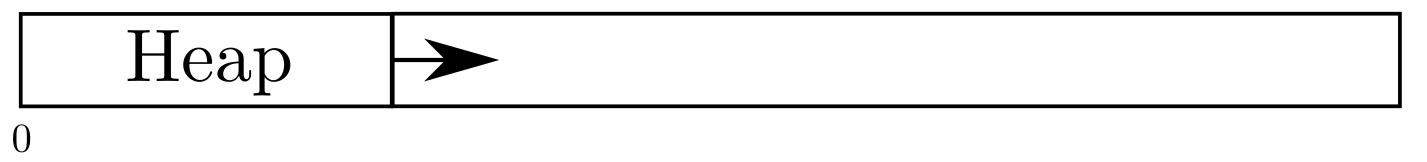
\includegraphics[scale=0.5]{regular_heap}
\caption{Typical WebAssembly memory layout}
\label{fig:wasm-heap}
\end{figure}


\subsection{Garbage collection}
OCaml is a garbage-collected language, so memory is managed automatically. However, memory is managed manually in WebAssembly, so a garbage collector must be implemented in the runtime system to manage objects allocated by compiled OCaml programs.

The two broad categories of garbage collectors are reference counting and tracing collectors. Reference-counting collectors keep a counter on each object for the number of pointers to that object that exist, freeing the object when the counter falls to zero. This has a high overhead, since a counter needs to be updated whenever a pointer is created or modified, and cyclic structures are never collected. Tracing collectors instead periodically scan a set of root objects that can be accessed directly, and use these to discover all objects indirectly reachable from them. Any object not marked as reachable is then safe to free. 

WebAssembly's implicit stack cannot be accessed directly, which complicates garbage collection as the values on the stack are part of the root set and need to be scanned during garbage collection. Therefore, garbage collection was left as an extension due to the challenges surrounding it. One solution is to implement a shadow stack in the linear memory, which stores a copy of each local variable saved on the implicit stack, allowing these to be traversed during garbage collection. Shadow stacks are more common in the context of security, where a function's return address is copied elsewhere in memory and compared when the function returns, detecting attempts to overwrite the return address on the stack \cite{shadow-stack}. % For performing garbage collection, a copy of each local variable is saved to the shadow stack, and garbage collection scans this region of memory to identify reachable pointers. 

The shadow stack must extend upwards from the start of the linear memory, since WebAssembly memory grows over time, so the top of the address space is not initially valid. Therefore, the top of the stack is limited by the starting position of the heap, and the layout of memory is as shown in figure \ref{fig:wasm-shadow}. %This is not a significant issue, as it was already possible to generate a stack-overflow error, by exhausting the available space in the underlying platform's implementation of the implicit stack. Using a shadow stack, the layout of linear memory is therefore as shown below:


%The WebAssembly memory now starts with the shadow stack, which can extend up to a fixed limit, after which the heap begins. This creates the possibility of a stack overflow error occurring, but such errors were already possible from the platform's implementation of the implicit stack, before garbage collection was added. It is not possible to have the stack and heap grow from opposite ends of memory, as typically happens in C, since the WebAssembly memory is initially small, so large blocks of memory would have to be copied to new locations when the memory grows. With garbage collection, memory therefore has the layout shown below:


% Mention the difficulties of garbage collection and the use of shadow stack
%The stack is managed implicitly, which is an issue for garbage collection since it means there is no way to scan the stack to discover which objects in memory are reachable. For this reason, garbage collection was left as an extension due to the challenges surrounding it. One way to solve this is to maintain a shadow stack in the linear memory, keeping a copy of each pointer stored on the stack so that this can be scanned instead. 


\hspace{-0.18cm}
\begin{figure}[H]
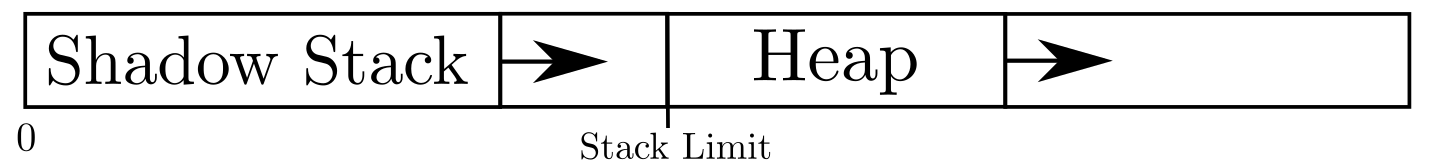
\includegraphics[scale=0.5]{gc_heap}
\caption{WebAssembly memory layout with a shadow stack}
\label{fig:wasm-shadow}
\end{figure}

% INCLUDE DIAGRAM OF HOW SHADOW STACKS WORK



%%%%%%%%%%%% ALL WRITTEN IN PRESENT TENSE FROM HERE ON, DOESN'T REALLY MAKE SENSE IN PAST TENSE? %%%

\section{Requirements analysis}
For this project to be successful, my compiler had to be able to compile OCaml programs that used just the integer, boolean, comparison and list standard-library operations, and did not use the module or object layers of the language, or exceptions. This defined the minimum subset of OCaml being supported. Achieving this required implementing multiple translation passes, first from the OCaml compiler's front-end output to my intermediate representation, and then from that to WebAssembly. I planned to verify the correctness of the translation passes by a set of test OCaml programs using the language features being supported. To be able to execute the resulting WebAssembly, I also needed to build a runtime system, to provide operations such as memory allocation. 

I had to collect data measuring the performance of the code output by my compiler, comparing it against the three alternatives mentioned previously. Performance would be measured in terms of execution time, heap usage, and the size of the compiled code. This required writing a set of benchmark OCaml programs, with equivalent programs in C and Grain, and these benchmarks should have reflected a range of programming styles. Testing scripts were also necessary to compile each of these benchmarks, for each alternative, and collect data for the three metrics identified. The aim was to demonstrate an improvement compared to the alternatives, particularly \jsofocaml{}, due to the inefficiencies of compiling OCaml to JavaScript mentioned in the introduction.


%allowing it to be compared with alternative methods for running code on the web.  Hopefully, this will demonstrate an advantage compared to \jsofocaml{}, since WebAssembly is a strongly typed binary format, so is expected to execute faster than the equivalent JavaScript when compiling a strongly typed language, such as OCaml.

Implementing optimisations in the compiler was chosen as an extension, to help achieve this improvement. This required a set of analysis and optimisation passes on both the intermediate representation and WebAssembly stages of the compiler. I also aimed to extend the range of OCaml programs supported by my compiler, as floating-point and reference operations increase the range of benchmarks that could be considered. %, and would make writing them easier. 

Another extension was to implement a garbage collector, using a shadow stack to make local variables accessible during garbage collection. This would allow more memory intensive benchmarks to be considered and make the comparison of my compiler against the alternatives more realistic, by not ignoring the overhead of memory management. %, which is not a part of my core requirements due to the challenges anticipated with garbage collection in WebAssembly.



\section{Software engineering methodology}

% Repetitive - just the same as the requirements analysis
The project can be separated into several stages that had to be completed in sequence, following the stages of a typical compiler pipeline and outlined in the requirements analysis. Translation from the IR to WebAssembly was performed in two smaller steps, and the runtime system was designed in parallel with the back-end of the compiler. Optimisations were only added once I had a working compiler, and could each be implemented independently. Since I used the OCaml compiler's front-end, my compiler was also written in OCaml, which helped improve my familiarity with the language features being implemented. Similarly, the runtime system was written in WebAssembly, except for the garbage collector, written in JavaScript due to its complexity and to allow modifying it more quickly. WebAssembly was the natural choice for interacting with programs compiled as WebAssembly, and again helped improve my understanding of the language.

This structure of mostly independent translation/optimisation passes lends itself to the Kanban methodology \cite{kanban}, which is an incremental approach to software development I have used before on team projects. Work was broken down into manageable tickets, most of which could be completed in a couple of days, building on the project incrementally. I used the Jira project-tracking platform from Atlassian to maintain a board of tickets \cite{jira}. Having a list of tasks in progress or blocked by other components, updated regularly, meant that elements of the project were not forgotten about and I could track how long each task was taking, identifying when a task was more complex than anticipated and needed to be further subdivided. The tickets were also a means of grouping ideas or issues with the pieces of work they affected, and I added more precise tickets to the backlog as the project progressed and it became clearer which elements to implement next.

%\subsection{Backups}

Both the project and dissertation were version-controlled using Git, backed up to GitHub daily and continually synced with OneDrive. %Commits were given meaningful commit messages, including the identifier of the ticket they were associated with, making it easier to navigate back to past changes if necessary. 
At the start of the project, I also checked that I could run the tools required, such as the OCaml and Grain compilers, on the MCS machines as a backup. 

%%%%%%%%%%%%%%%%%%%%%%%%%%%%%%%%%%%%%%%%%%%%%%%%%%%%%%%%%%

%The implementation of the compiler can be cleanly separated into building a minimal working compiler, and adding optimisations on top of that. The first of these lends itself to an incremental development strategy, as a compiler can be split into several key stages where the interface from one stage to the next significantly affects the complexity of the next stage. A compiler is typically divided into a front-end for parsing and type-checking, a middle-end for translation to a suitable intermediate representation and performing optimisations, and a back-end for generating WebAssembly code. I ultimately determined that my compiler should have two separate IRs, and so worked through these stages one at a time, starting from the typed output of the OCaml compiler front-end. 

% Also added language features this way
%After achieving a working compiler, iterative design becomes far more practical since I cannot accurately predict the benefit of different optimisations without repeated data collection on a range of benchmarks. For both stages of development, I decided to use a Kanban board to keep track of tasks. % By associating segments of work to numbered tickets, it would be easier to find specific changes once far into the project. 
%By keeping a backlog of tickets, this was an easy way to track extra features that needed implementing as I developed the compiler, and to keep ideas and issues grouped by the piece of work they affected. It also meant that I could see how long I had been working on each ticket, which was useful for identifying the tasks I needed to dedicate more time to or subdivide into more manageable tasks.

%\subsection{Tooling}

\subsection{Testing}
% Primarily test-driven development with Ocaml unit test samples for each feature. Sort of an integration test
% TODO: Specific unit tests for mock IR programs to check specific components e.g. free vars, number of locals needed
% More specific tests to check that optimisations handle complex cases correctly.
Language features were added to the compiler following test-driven development. Before adding a new primitive, language construct or optimisation, OCaml programs would be written using that feature, and the output of the OCaml interpreter on those files would be recorded. 
I wrote a script to compile and run each of these programs with my compiler, comparing their output with the expected values. This ensured that each new feature was implemented correctly, and that a change or new optimisation did not break any of the previous tests. % Additional tests were also added as I considered edge cases while implementing features, ensuring that they were not overlooked by future modifications.
Additionally, for tests added to verify that optimisations were performed safely, inspecting the output WebAssembly ensured that optimisations were being performed in the correct places. 

% The same process was helpful for ensuring optimisations were only performed where safe to do so, adding cases where incorrectly applying a transformation would break the program. This was most often where expressions in the program had side-effects that must be preserved, preventing some optimisations being applied.

%Optimisations were similarly tested against all prior test programs, and additional tests were added for where these optimisations were more likely to make a mistake. % More detail in implementation section?

Unit tests were written with OUnit \cite{ounit} for several of the utility functions involved in translation and optimisation. For example, checking that the free variables in IR programs  were computed correctly, or that removing an instruction from the flowgraph representation of a WebAssembly program correctly preserved the edges linking that node's successors and predecessors.


Testing whole translation passes was challenging, since translation often introduces several inefficiencies whilst still being correct, and the translation cannot be verified without running the full compiler pipeline and executing the output. Therefore, until the core stages of the compiler and runtime were built, I relied on pretty-printing code to display the intermediate representations for some sample programs. This allowed identifying any obvious errors by inspection, and was only relied on at the start of the project, before even a minimal pipeline had been written.
 %. Although this was unlikely to detect subtle errors, it was only relied on at the start of the project, when even a minimal pipeline did not yet exist.


% Should go at the top as this was the first form of testing?
% TODO: Is this worth mentioning? Probably the first thing I want to cut out
%Testing individual stages of translation was challenging, since the intermediate representation produced would generally have several inefficiencies that later optimisation passes would remove, so could not be directly compared against some expected output. Similarly, trying to write an interpreter for the IR output would be time consuming and error prone. As such, I checked the initial stages of my compiler were behaving as expected by adding pretty-printing code for the intermediate representations, and manually inspecting the output for a few simple test programs. This would highlight any significant errors, and was only necessary until a minimal compiler pipeline down to WebAssembly was implemented, making testing much easier.

%Unit tests were still written with OUnit \cite{ounit} for specific functions involved in translation, which could be verified in isolation. For example, manually building the IR or WebAssembly representation of a program, and verifying properties such as which variables are free in a function body, or which variables are live at each point in the body. The distinction here is that, while there is flexibility in the code produced to perform the operations described by a previous representation, the analyses used during translation have a precise meaning that can be verified. 

%Testing individual translation stages was challenging since I did not want to spend a large amount of time writing an interpreter for my IR, which would itself be prone to errors in handling the semantics of the IR, and checking the exact output of the translation would be impractical as the unoptimised compiler would introduce several unnecessary assignments and checks. Therefore, I initially checked these stages by adding pretty-printing code for the IR and manually inspecting the output for some of the test programs. The simplifications made by each IR made translated programs relatively easy to follow, and this was only necessary until the minimum compiler pipeline was implemented, then programs could be run as WebAssembly and be tested much easier. \\
% TODO: ACTUALLY DO THIS!
%I still wrote unit tests for the more complex utility functions involved in translation, which could be more easily verified. This included tests for identifying the free variables of a block of code (important for constructing closures) and for the number of separate values allocated at once (important for determining the number of local variables a function requires). This should be inflexible values so are not affected by the compiler initially being inefficient, hence later optimisations would not invalidate these tests.


\subsection{Tools used} % REFERENCES TO EVERYTHING
I worked on the project on my Windows laptop, using Windows Subsystem for Linux to run OCaml. Opam, the OCaml package manager, was used to manage the 
OCaml compiler and packages needed for the project. I used the OUnit package for writing unit tests, the Wasm package for some of the back-end functionality, such as %a data structure representing WebAssembly modules and 
utility functions to output WebAssembly to a binary file, and the \jsofocaml{} package as an alternative to my compiler. The project used the front-end of version 4.11.1 of the OCaml compiler, which was the latest version at the start of the project, although version 4.12.0 has since been released. 

% Unnecessary to mention Grain/Clang? Already brought up a few times as alternatives

I used the WebAssembly Binary Toolkit to translate between the binary and text format, both for producing a binary of the runtime system, and to inspect the output of my compiler on test programs. Node.js was used to run the output WebAssembly and perform benchmarking, and the project was developed using the IntelliJ IDE, available under its educational license.


\section{Legality}
I used of the front-end of the official OCaml compiler \cite{ocaml}, which is distributed under the GNU Lesser General Public License. My use of the compiler and modifications to it are therefore permitted, provided that I retain the original licence in my project and highlight where modifications have been made. 

Benchmark programs were adapted from two existing sources \cite{chris00, benchmark-game}, one of which is also distributed under the GNU LGPL, and the other under the BSD-3 licence. Therefore, modification is once again permitted, provided the original licences are retained.





%This chapter covers relevant (and typically, recent) research
%which you build upon (or improve upon). There are two complementary
%goals for this chapter:
%\begin{enumerate}
%  \item to show that you know and understand the state of the art; and
%  \item to put your work in context
%\end{enumerate}

%Ideally you can tackle both together by providing a critique of
%related work, and describing what is insufficient (and how you do
%better!)

%The related work chapter should usually come either near the front or
%near the back of the dissertation. The advantage of the former is that
%you get to build the argument for why your work is important before
%presenting your solution(s) in later chapters; the advantage of the
%latter is that don't have to forward reference to your solution too
%much. The correct choice will depend on what you're writing up, and
%your own personal preference.



\clearpage
\chapter{Implementation}

\section{Administrative Normal Form}
% Reference for ANF?
From OCaml's Typedtree data structure, the first pass of the compiler translates programs to administrative normal form (also called A-normal form or just ANF), which linearises the syntax tree so that the operands to operations are always constants or idnetifiers, with the exception of control flow construsts such as if/while statements. For example:

\begin{verbatim}
f(g(x), h(x+y))
\end{verbatim}
would be translated to
\begin{verbatim}
let v0 = g(x) in
  let t = x + y in 
    let v1 = h(t) in
      f(v0, v1)
\end{verbatim}

Temporary values are now explicit and the linear structure makes optimisations such as common subexpression elimination and dead assignment elimination easier to implement in this form. Code which may execute zero or many times cannot be completely linearised, for example the subexpressions for the body of a while loop must be evaluated within the while loop, since they are never evaluated if the condition is false. \\
Linearising is implemented using three mutually recursive functions which compile immediates (constants/identifiers), compound terms such as \verb|x + y|, and top level terms such as \verb|let x = e in e'| or \verb|e; e'|. The first two of these return a pair of the actual term needed, and a list of any setup operations extracted as part of linearising the expression being compiled. Compiling a top level term then converts this result and list of setup operations into a tree which performs all of the setup then evaluates the result.
% Give actual examples of code translation/algorithm cases?
% OCaml primitives handling?

This is achieved by translation to the \verb|Linast| (Linear AST) datatype, which also replaces patterns in the Typedtree with the code needed to evaluate them. This includes combining the cases of a match or function into a single expression, making use of switch statements on integers where possible. Pattern matching was initially done with a naive method of trying each pattern in sequence, moving on to the next if that failed. \\
% How much to explain vs just reference the paper? Not my ideas so no marks to be gained, or want to show complexity for implementing difficult algorithm?
Once a working compiler was achieved, this was replaced with a more efficient approach which is the first algorithm described by Fessant and Maranget \cite{ocamlpatternmatch}.  The idea is to represent each pattern as a row of an $n \times m$ matrix, with an action associated with each row in the event that pattern matches, and a vector of values to perform pattern matching against. Pattern matching is then divided into a number of cases based on the first column of the matrix. For example, if every pattern in the first column is a constructor pattern, the matrix can be 'specialised' for each possible constructor. This involves filtering out only the rows $c(q_1, \dots, q_k) \ p_2 \ \dots\ p_m$ which match a constructor $c$, then unwrapping the sub-patterns to get new rows $q_1 \ \dots\ q_k \ p_2 \ \dots\ p_m$. This gives the matrix to use for pattern matching, after a switch statment determines that the first values is constructor $c$, so doing this for each possible constructor will give a switch statement which performs pattern matching. 

% Guards?

%%%%%%%%%%%%%%%%%%%%%%%%%%%%%%%%%%%%%%%%%%%%%%%%%%%%%%%%%%%%%%%%%
\section{Compiling Identifiers}
After any optimisations are performed, the linearised tree is then compiled to a lower intermediate form. The tree is replaced with a list of instructions, and identifiers are resolved into integer indexes for argument, local, global or closure bound variables. 
% Give more detail about blocks in WebAssembly
Conversion to a list of instructions is straightforward since WebAssembly contains nested blocks. \verb|Block| constructs in WebAssembly contain a list of instructions and introduce a label at the end of the block, which can be jumped to from within the block. \verb|If| blocks are similar but contain two lists of instructions, and \verb|Loop| blocks have the label at the start of the block, allowing code to be repeated. 
Rather than map to these straight away, programs are still described using \verb|if| and \verb|while| constructs, which are easily mapped to WebAssembly at the code generation stage. % Put examples when we get there, not here

This stage also lifts any function declarations to the top level of the program, since closures and environments are now explicit, so the result is a list of functions. The complexity here is in determining the free variables of a function and the number of local stack variables needed by the function body, both of which are done by simple recursive algorithms. The number of locals needed is the maximum needed at any point in the function body. This increases by one after each let binding is evaluated, and for loops also require two to remember the current and end values for the loop (for loops in OCaml have a very constrained \verb"for var = i [up|down]to j do ... done" syntax). 

% Currying removed at this point. Wasn't being used anyway so why do I allow it at all? Does it actually provide any benefit to me?

\section{Code Generation}
WebAssembly generation is then straightforward, as each of the constructs and primitive operators in my lower IR are all simple to implement. The variable bindings in the lower IR were separated into argument, local, global and closure bindings. Argument and global bindings translate directly to Local and Global operations respectively. The locals in a function are laid out as function arguments, then swap space locals used to implement some of the operations in WebAssembly, then locals allocated above for let bindings and loops. Therefore, local bindings are offset by the number of swap spaces and function arguments. The first argument to each function is its closure, so closure bindings first get local 0 then do a load from that address, with an offset selecting the correct variable from the closure. 

I also wrote a runtime in WebAssembly providing functions for memory allocation, polymorphic comparison, boxing of floats in memory, and list append and some of the integer primitives. These are declared as imports to the WebAssembly module and each function index in my IR must be offset by the number of runtime functions imported. Additionally, the memory for the module is also imported from the runtime since it is managed by the allocation function from the runtime imports. Lastly, each of the globals and functions from the module is exported. Every function is exported so that values representing closures can be returned from WebAssembly. As integers are encoded by shifting them left by one, and so that pointers to closures can be used to call functions in WebAssembly from JavaScript, I added a JavaScript wrapper which uses knowledge of how values are represented in memory to be able to pass values back into compiled functions, or return integer values back to a JavaScript caller.

Although I did not implement a garbage collector, data still needed to be tagged to identify its type so that OCaml's \verb|compare| function, which is defined on all types, would work correctly. As every operation is on either 32-bit integers or 64-bit floats, pointers are always aligned on 4-byte boundaries so the last 2 bits are not needed. I therefore tag integers as 10 or 00 by shifting them left one, function as 11, and other blocks from tuples or constructors as 01. In the last case, data blocks are represented as a variant tag, their arity, then the elements they contain. As OCaml limits the number of different constructors supported% Reference required
, the variant tag is guaranteed to be a non-negative integer. Therefore, -1 was used to encode floats, which were separately represented as -1 followed by the 64-bit float value. This is necessary since the arguments and return values of WebAssembly functions are strongly typed. Therefore, all functions take a 32-bit integer which is decoded as an integer or pointer to data or a float as required by the body of the function.

% Describe graphs






%This chapter may be called something else\ldots but in general
%the idea is that you have one (or a few) ``meat'' chapters which
%describe the work you did in technical detail.

\clearpage
\chapter{Evaluation}
This chapter compares the performance of my compiler with three existing alternatives for running code on the web: Compiling C to WebAssembly with Clang/LLVM, compiling Grain (a functional language based on OCaml that compiles to WebAssembly), and translating OCaml programs to JavaScript with the Js\_of\_ocaml tool.
I also measure the impact of the optimisations implemented in my compiler. Performance is based on three metrics: 

\begin{itemize}
\item \textbf{Execution time}: This is measured by a JavaScript program, run using Node.js, for each of the alternatives. Timing information is obtained from the \verb|performance| interface, which has up to microsecond precision and is not affected by system time changes, so is guaranteed to be monotonic \cite{timing}. This is sampled over 20 runs of the program and the mean and 95\% confidence interval are recorded. 

\item \textbf{Heap usage}: The heap memory used is also collected by these scripts. Without garbage collection, my runtime allocates memory linearly so a call to allocate 0 bytes returns the total memory used. For the garbage-collected allocator, I created a separate version that tracks the peak memory allocated, updating this on each allocation. 

The Grain runtime's development build outputs similar memory-tracing statistics, including the amount of heap memory used. 
The overhead of tracing is significant so this is done separately to collecting timing information. For C, where parts of \verb|stdlib| are included in the WebAssembly output for memory allocation, \verb|sbrk(0)| returns the size of the WebAssembly linear memory used. % Mention 64KiB resolution?
Lastly, for programs translated to JavaScript, the benchmarking script is run with the \verb|--expose-gc| option. This allows calling the garbage collector before the program is executed, and obtaining the memory used by calling \verb|process.memoryUsage().heapUsed| before and after the program runs. This is an approximate value, so it is also averaged over 20 iterations.

\item \textbf{Output file size}: This is easily obtained from the file system.

\end{itemize}

\newpage
\section{Microbenchmarks}
I wrote a set of test programs, each aiming to represent a different programming style, to see how performance varied across applications. The programs were also parameterised so that comparisons could be made at different problem sizes. % Only a few instances of this are included in the data to keep the number of dimensions of comparison manageable, instead focusing more on other aspects. The microbenchmarks used were:
Where available, these programs were based on code from existing benchmarking libraries.

% TODO: Rename everywhere so I can use other names instead
\begin{itemize}
\item \verb|alltrees|: Constructs a list of all binary trees of a given size, which is very memory intensive. % and objects that exist for varying lifetimes.

\item \verb|arith|: Computes Euler's totient function for all integers from 1 to a given \verb|n|, involving a large amount of integer arithmetic. This was based on problem 34 of the 99 Problems in OCaml \cite{99-problems}.%, implementing Euler's totient function.

\item \verb|composition|: Constructs a function which is the composition of a list of simple functions and maps it over a list, making heavy use of higher-order functions.

\item \verb|funcrec| (functions, records): Compares three forms of parameterisation: Using functions defined at the top-level of a program, passing those functions as arguments, and passing those functions as fields of a record argument. This was based on an existing repository of OCaml benchmarks available on GitHub \cite{chris00}.

\item \verb|mergesort|: Implements mergesort, making heavy use of lists and pattern matching.

\item \verb|nbody|: Simulates the n-body problem, simulating the motion of planets for a number of time steps and making heavy use of floating-point arithmetic. This was adapted from the version in the Computer Language Benchmarks Game repository \cite{benchmark-game}.
\end{itemize}

%A couple other microbenchmarks were also used to demonstrate the worst-case behaviour some optimisations aim to avoid. These will be described later when the data for those optimisations is presented. 


\section{Comparison against alternatives}
Although most of the runtime for my compiler is written in WebAssembly, the garbage-collected memory allocator is written in JavaScript due to its complexity and wanting to make several improvements to it. Therefore, the performance of my compiler is indicated with and without garbage collection (labelled as `OCaml' and `OCaml GC'), to distinguish the overhead of calling between WebAssembly and JavaScript for each memory allocation. The data given is also for the optimised version of the compiler.

In the following graphs, the output of compiling equivalent C programs to WebAssembly with Clang/LLVM is labelled as `C', and the output of compiling Grain to WebAssembly is labelled as `Grain'. Lastly, the JavaScript programs produced by translating the OCaml benchmarks with Js\_of\_ocaml are labelled as `JS'. The subscript value on the names of benchmarks indicates the problem size, where multiple instances of the same benchmark were included.

\subsection{Execution Time}

\begin{figure}[H]
\hspace{-0.7cm}
\includegraphics[scale=0.42]{figures/alternatives_timing2}
\vspace{-0.5cm}
\caption{Execution times for each alternative (lower is better)}
 \label{fig:alt_timing} 
\end{figure}

In figure \ref{fig:alt_timing}, we see that the execution speed can vary by a couple orders of magnitude between the least and most efficient method. Unsurprisingly, the programs translated to C by hand and compiled to WebAssembly are the fastest. At the opposite end, Grain is always significantly slower than the other methods. My compiler is always faster than the equivalent JavaScript when run without garbage collection, however the overhead of garbage collection results in the two being more balanced, as shown further in figure \ref{fig:js_oc_timing}.% performing better on some programs and worse on others. This is shown in more detail below:


\begin{figure}[H]
\hspace{-1.6cm}
\includegraphics[scale=0.52]{figures/js_ocaml_timing}
\vspace{-0.5cm}
\caption{Comparison between my compiler and Js\_of\_ocaml}
 \label{fig:js_oc_timing} 
\end{figure}

Without garbage collection, my compiler's output	executes between 0.33 and 20 times faster than the JavaScript program produced by  Js\_of\_ocaml. With garbage collection, execution time grows much faster with problem size and my compiler performs worse for programs making a large number of memory allocations.

%it still outperforms the JavaScript alternative in most cases, except for programs making a very large number of memory allocations such as \verb|alltrees| with a large problem size.


\subsection{Heap usage}

\begin{figure}[H]
\hspace{-1cm}
\includegraphics[scale=0.43]{figures/alternatives_heap2}
\vspace{-0.5cm}
\caption{Heap usage for each alternative (lower is better)}
 \label{fig:alt_heap} 
\end{figure}

There are no bars for C for \verb|arith|, \verb|funcrec| and \verb|nbody| in figure \ref{fig:alt_heap}, as these did not require the heap to implement. 
% TODO: Should try to get some value for Grain Arith_1000, even if very few iterations
There is also no data for Grain for \verb|arith_1000| as the program did not appear to terminate with tracing enabled.
% was very slow without tracing (see figure \ref{fig:alt_timing}) and with tracing enabled did not terminate after 10 minutes.

For the compiled C programs that did use the heap, my garbage-collected runtime only uses more memory for \verb|mergesort|, where my implementation uses 70\% more memory at the larger problem size. This difference is due to C being an imperative language, with manual memory management, where it is natural to implement \verb|mergesort| to perform operations in-place. Although manual memory management allows more precise control over memory, it also adds to the complexity of writing programs.
The WebAssembly memory is initialised as 2 pages (128KiB), which is the size recorded for \verb|composition| and \verb|mergesort|$_{1000}$, indicating that these programs may need less memory than the amount initially allocated.


%Where the compiled C programs did use the heap, my garbage-collected runtime uses at worst 35\% more memory. However, C is not a garbage-collected language, so additional effort is required when writing the programs, to perform manual memory management. 
My implementation uses significantly less memory than both the JavaScript and Grain alternatives. In every test, % (ignoring the Grain result for \verb|arith_1000|), 
the garbage-collected runtime uses at most one third of the memory used by either the JavaScript or Grain version. 
% NEW - DESCRIBING MEMORY MANAGEMENT IN EACH OF THE ALTERNATIVES
The Grain compiler has its own runtime system for managing WebAssembly memory, whereas Js\_of\_ocaml converts OCaml programs to JavaScript, which then rely on the garbage collector of the environment the benchmarking script is executed in. I ran the tests with Node.js, so this used Chrome's V8 JavaScript engine.


For my compiler, the garbage-collected runtime uses more memory for \verb|arith| and \verb|funcrec| than the version without garbage collection.
These tests have fewer opportunities for garbage collection so it saves little memory, but the implementation consumes more memory with garbage collection due to the overhead of headers and trailers on allocated blocks. In the worst case, \verb|funcrec| has no opportunities for garbage collection and almost exclusively allocates small objects of 8 bytes. Since each header and trailer is 8 bytes, garbage collection triples the amount of memory used.



\subsection{Output File Size}

\begin{figure}[H]
\hspace{-1.2cm}
\includegraphics[scale=0.5]{figures/alternatives_size2}
\vspace{-0.8cm}
\caption{Output size for each alternative (lower is better)}
 \label{fig:alt_size} 
\end{figure}

As expected, figure \ref{fig:alt_size} shows that the JavaScript output tends to be largest, as JavaScript is a text format rather than a binary format like WebAssembly. On average, it is 8 times larger than the output of my compiler with garbage collection enabled. Grain also produces much larger binary files, averaging about 3.5 times larger than my compiler's output. Inspecting the compiled output, there appear to be a few reasons for this. First, programs import a larger set of functions from Grain's runtime than used by my compiler. It also uses a reference-counting garbage collector, which adds more overhead since updating a variable requires both incrementing the new value and decrementing the old value, whereas my garbage collector just overwrites the old value on the shadow stack. Lastly, it does not appear to optimise the WebAssembly produced, compared with my compiler, which uses a register-allocation algorithm to reduce the number of local variables declared, and peephole optimises trivially useless statements such as \verb|local.get i; drop|.

Compared with the output of compiling a C program, the sizes are similar except where parts of \verb|stdlib| have to be included for memory allocation, which makes those programs about 9KB larger. For comparison, my runtime without garbage collection is a 740B WebAssembly file, but the garbage collector is implemented in JavaScript, which when minified is a 4KB file.

% CAREFUL! MANUALLY SET REFERENCES! MAY CHANGE IF CHAPTERS REORDERED/REMOVED!
Figure \ref{fig:alt_size} also demonstrates the overhead of garbage collection in terms of the extra bookkeeping operations added to maintain the shadow stack. %described in section 3.6.1.
On average, this adds about 30\% to the size of the output WebAssembly. % Tim said ``REFER BACK''? WHAT DOES HE MEAN BY THAT? Possibly meant paragraph below

\section{Optimisations}

I first compare the impact of the IR and WebAssembly optimisations described in section 3.5, and their combined effect on performance. After that, I look at the impact of specific optimisations at the IR level by seeing how performance changes when one is removed, and the benefit of optimising pattern matching. Finally, I show the benefit of repeating the optimisation passes multiple times. %, as well as looking at how the phase ordering at the IR level impacts performance.  -- LEAVE THIS FOR IF SECTION TOO SHORT

Data is collected with garbage collection disabled to exclude the overhead it introduces, which depends primarily on the garbage collection implementation used by the runtime system, rather than how programs are optimised.

\subsection{IR and WebAssembly optimisations}
\vspace{-0.4cm}
\begin{figure}[H]
\vspace{-0.05cm}
\hspace{-0.8cm}
\includegraphics[scale=0.47]{figures/opts_threeplots2}
\vspace{-0.7cm}
\caption{Performance with IR and WebAssembly optimisations}
 \label{fig:opts} 
\end{figure}
The peephole optimisations done at the WebAssembly level have no impact on memory usage or execution time, but consistently reduce output size by about 10\%, as shown in figure \ref{fig:opts}. The IR optimisations reduce execution time and heap usage by at least 30\% for all microbenchmarks, except \verb|nbody|. \verb|nbody| is the only program which does not improve in all metrics, most likely because it is an imperative-style program and the optimisations implemented are unable to optimise uses of mutable variables.
% and instead executes 3\% slower. It is an imperative-style program, which may explain why the optimisations perform well on the other programs but not on it, since they are unable to optimise uses of mutable variables and \verb|nbody| has no recursion to optimise either. 
 For \verb|arith| and \verb|funcrec|, inlining or rewriting functions has completely removed the need to construct closures recursively, resulting in near zero heap usage. %The execution time of \verb|nbody| is the only case where optimisations decrease performance, but only by 3\%.  \verb|nbody| is an imperative style program, which may explain why the optimisations perform well on the other programs but not on it, since they are unable to optimise uses of mutable values and \verb|nbody| has no recursion to optimise.

\subsection{Impact of inlining, uncurrying and tail calls}
\vspace{-0.4cm}
\begin{figure}[H]
\hspace{-1.5cm}
\includegraphics[scale=0.5]{figures/specific_opts2}
\vspace{-0.8cm}
\caption{Impact of individual optimisations}
 \label{fig:specific-opts} 
\end{figure}

Figure \ref{fig:specific-opts} shows the change when one optimisation is removed, so the magnitude of each bar can be viewed as the speed-up or size reduction an optimisation has, on top of the optimisations already present. First, inlining only increases file size in one case, \verb|funcrec|, and only by 5\%, so the optimisation does not cause significant code bloat. Instead, inlining reduces the size of the output in cases where it completely removes a function definition. Overall, it has a relatively small impact on performance, with the biggest change being a 15\% speed-up for \verb|funcrec|. This suggests that the heuristics used for inlining may be too conservative. However, these are all relatively small benchmark programs, which could also limit how significant a change can be achieved by inlining. % suggesting that either the heuristics for inlining were too restrictive or that this set of microbenchmarks or other optimisations are not complex enough to see significant improvements from inlining.

% Getting too specific? Talk in higher-level general details?
Tail-call optimisation does not affect most of the programs, but improves the execution speed of \verb|funcrec| and the speed and file size for \verb|arith|. A more important factor, not shown by figure \ref{fig:specific-opts}, is that tail-call optimisation allows some programs to execute that would otherwise give an error, for example: \\
\verb|let rec f x = if x = 0 then 0 else f (x-1)| \\
Despite being a very simple function, without tail-call optimisation, \verb|f(30000)| exceeds the maximum call-stack size and the program fails. With tail-call optimisation, the function no longer makes recursive calls so can handle any input size.

Lastly, uncurrying fully applied functions has the most significant impact on performance. None of the benchmarks are negatively impacted by it and most speed up, by up to 50\%. Additionally, not having to construct a closure for each separate argument reduces the amount of space used on the heap, and the number of functions defined in the code. In the case of \verb|arith|, this removes the need to recursively construct any closures, so heap usage no longer increases with problem size. Once again, \verb|nbody| is not improved, as it lacks opportunities for this optimisation to be applied.

\subsection{Pattern Matching}
\begin{figure}[H]
\includegraphics[scale=0.7]{figures/patterns}
\vspace{-0.8cm}
\caption{Impact of optimised pattern matching}
 \label{fig:patterns} 
\end{figure}

For evaluating the optimisations to pattern matching, I consider an additional microbenchmark, \verb|pattern|, which repeatedly calls each case of the function below, and benefits from the context information described in section 3.2.1.
\begin{verbatim}
type lst = Nil | One of int | Cons of int * lst

let f l1 l2 = match (l1, l2) with
  | Nil, _ -> 0
  | _, Nil -> 1
  | ((One _, _)|(_, One _)) -> 2
  | Cons _, Cons _ -> 3
\end{verbatim}
%This set of patterns benefits significantly from the reordering of cases  and use of context information described in section 3.2.1.


As figure \ref{fig:patterns} shows, the optimisations have little or no impact on benchmarks with only simple patterns, but reduce output size for \verb|mergesort| and \verb|pattern|, which both involve more complex pattern matching. Execution time is also reduced slightly for \verb|pattern|.
This shows that the optimisations provide a slight benefit for complex pattern matching, without having a negative impact in simpler cases.

% This shows that, although the difference will often only be small, the changes to pattern matching can improve performance for programs with complex patterns, without reducing performance in simpler cases.

\subsection{Impact of number of iterations}
%Only one instance of each benchmark is shown, as the pattern is identical for other problem sizes.
\vspace{-0.5cm}
\begin{figure}[H]
\hfill
\includegraphics[scale=0.62]{figures/iterations} \hfill
\vspace{-0.3cm}
\caption{Effect of repeating optimisation passes}
 \label{fig:iterations} 
\end{figure}

Figure \ref{fig:iterations} demonstrates that, in almost all cases, there is no further improvement after each optimisation pass has been performed three times, so this was chosen as the default number of iterations for all other tests. This ensures that every optimisation happens both before and after every other one, so the effects of phase ordering are reduced. % This is helpful since there are several passes being performed at the IR level, so much more data and analysis would be necessary to select the best permutation of them with any confidence.
Multiple iterations can also benefit one optimisation in isolation e.g. \verb|let y = x in let z = y in f(z)|. The first pass of propagating variables would replace \verb|f(z)| with \verb|f(y)|, but another pass is needed to replace this with \verb|f(x)|, allowing both \verb|y| and \verb|z| to be removed.

% TODO: Phase ordering or not?


\section{Garbage Collection}
\vspace{-0.5cm}
\begin{figure}[H]
\hspace{-2.8cm}
\includegraphics[scale=0.53]{figures/three_gcs}
\vspace{-0.6cm}
\caption{Effect of changes to garbage collection}
 \label{fig:three_gcs} 
\end{figure}

Figure \ref{fig:three_gcs} shows that, due to adding a trailer to every memory allocation (described in section 3.6.3), the modifications to garbage collection increase both execution time and memory usage for most of the microbenchmarks, since these are small programs that generally only require simple memory management. 

\begin{figure}[H]
\hfill \includegraphics[scale=0.75]{figures/mal} \hfill
\caption{Performance on fragmented memory}
 \label{fig:mal} 
\end{figure}

Figure \ref{fig:mal} demonstrates the benefit of these changes for a program allocating data after memory has been fragmented. The function below interleaves allocations to three different lists, one of which contains \verb|Cons2| cells which are larger than \verb|Cons1| cells. After the \verb|shortFreedList| and \verb|longFreedList| are discarded and garbage collected, the heap has lots of fragmented free blocks, with every tenth block being large enough for a \verb|Cons2| cell. 
\begin{verbatim}
type list = Nil | Cons1 of int * list | Cons2 of int * int * list

let longLivedList = ref Nil
let shortFreedList = ref Nil
let longFreedList = ref Nil

let rec buildLists = function
  | 0 -> ()
  | n ->
   (if (n mod 20) = 0
      then longFreedList := Cons2(n, n, !longFreedList)
    else if (n mod 2) = 0
      then shortFreedList := Cons1(n, !shortFreedList)
    else 
      longLivedList := Cons1(n, !longLivedList));
    buildLists (n-1)
\end{verbatim}
The problem size in figure \ref{fig:mal} refers to how many times those larger blocks are reallocated. The original implementation scans the free list so considers nine small blocks for every one larger block it can allocate, and scans over all of the smaller free blocks before calling garbage collection. Binning free blocks by size avoids this, and the modified version only considers blocks that are large enough to allocate, running 50\% faster. 

Memory is initially one large free block, and fragmentation is only an issue once this large block is nearly all allocated, otherwise allocations continue to be taken from the large block rather than scanning the free list. The modified version adds a trailer to each block, so fragmentation is often an issue at different points for each version, since they consume a page of WebAssembly memory after a different number of allocations. Therefore, it was necessary to construct this artificial example of fragmentation, demonstrating the effect it has for both versions.

\subsection{Threshold to not grow memory}

Figure \ref{fig:speedup} demonstrates the benefit of having a threshold for garbage collection, increasing memory whenever garbage collection fails to free more than 1KiB of memory, not just when it fails to free a block of the required size. As problem size grows, \verb|alltrees| gets more memory intensive and the modified version begins to narrowly outperform the original. However, the improvement with the threshold is much more significant, surpassing 40\% at the largest problem size.

\begin{figure}[H]
\hfill \includegraphics[scale=0.75]{figures/speedup} \hfill
\vspace{-0.2cm}
\cprotect\caption{Performance on \verb|alltrees|}
 \label{fig:speedup} 
\end{figure}


\begin{figure}[H]
\hfill \includegraphics[scale=0.88]{figures/traces2} \hfill
\vspace{-0.8cm}
\caption{Objects freed during execution of \texttt{alltrees}}
 \label{fig:traces} 
\end{figure}

Figure \ref{fig:traces} reveals why this is the case, by examining a trace of the number of objects freed each time the garbage collector runs, and the total number of garbage collections performed before the program terminates. There is a trend in the number of objects being freed to decrease over time, as the number of long-lived objects grows, until eventually memory has to grow and a large number of allocations occur before the next garbage collection, hence the spikes in the traces. 

We see an identical pattern both with and without the threshold, but this pattern is compressed when the threshold is used, in which case the program performs about 25\% fewer garbage collections in total.  
Rather than having tails of inefficient garbage collections, the threshold results in many objects all begin freed in one pass the next time garbage collection runs, after the newly-requested memory is used up many allocations later. This results in the garbage collector being invoked fewer times in total, without requesting memory in cases where it would otherwise not be necessary. The value of 1KiB was selected based on the amount freed by these tails of inefficient collections.

\section{Summary}
I have shown how my compiler compares to existing methods of running code on the web, outperforming Grain and Js\_of\_ocaml in many instances. I have also demonstrated the cases where my optimisations improve performance, and given possible explanations for the behaviour observed.














%For any practical projects, you should almost certainly have
%some kind of evaluation, and it's often useful to separate
%this out into its own chapter.

\clearpage
\chapter{Conclusion}

This project met its success criteria, supporting the core OCaml language with integer, boolean, comparison and list operations, as well as all OCaml's control-flow and pattern-matching constructs, besides exceptions.

I also implemented extensions in each of the directions identified at the start of the project. The subset of OCaml supported was extended with references and basic floating-point operations, and the compiler supports using .mli interface files to hide parts of programs in the compiled WebAssembly.
Several optimisations were implemented, including function inlining, uncurrying and tail-call optimisation, as well as clean-up passes on the intermediate representation and WebAssembly.
I also extended the runtime system with a mark-and-sweep garbage collector, using a shadow stack due to the WebAssembly stack being implicit.% overcoming not being able to scan the WebAssembly stack by implementing a shadow stack in the linear memory. 
%Past projects compiling functional languages to WebAssembly have mentioned garbage collection as an extension that was not implemented, so this project has achieved something new in that respect.

With these optimisations, my compiler consistently produces smaller output files than the Js\_of\_ocaml tool, and the compiled programs consume at most one third the amount of memory. 
This demonstrates the benefit of compiling a strongly typed language, such as OCaml, to WebAssembly, avoiding the inefficiencies of JavaScript. Execution time was also reduced, but only for benchmarks that did not make heavy use of the heap.


\section{Personal reflection}
This project allowed me to learn more about how complex language features can be implemented, such as pattern matching and mutually recursive functions, which were not discussed in the Part IB Compilers course. It has also reinforced the importance of careful planning and preparation for substantial software projects, which allowed me to complete the core compiler relatively quickly and explore a range of interesting extensions. 

I was able to work much faster during the breaks than in term time, due to not having units of assessment and lectures to balance with the project. My initial plan accounted for the unit of assessment exam taking priority the week it was set, but could have allocated more work during the breaks. As a result, I implemented benchmarks and data collection during the Christmas break, a couple weeks ahead of schedule, and mostly focused on extensions during Lent term.



%%%%%%%%%%%%%%%%%%%%%%%%%%%%%%%%%%%%%%%%%%%%%%%%%%%%%

%Whilst I worked at a steady pace both during term time and in the breaks, the timetable in my project proposal should have put greater emphasis on having more time available during the breaks. I implemented benchmarks and data collection during the Christmas break, a couple weeks ahead of schedule, and mostly focused on extensions during Lent term, which could have been better anticipated in my initial plan.

%Whilst I managed to work at a steady pace both during term time and in the breaks, always staying on track or ahead of schedule, my original timetable did not account for me being able to allocate much more time to the project during the breaks.
%This led to me being about three weeks ahead of schedule at the start of Lent term, which meant I had lots of time to work on extensions, but had to come up with new goals for when I wanted to complete components by, that could have been present in my initial plan.


% NEW BIT - LESSONS LEARNT
% PROBABLY FAR TOO LONG WITH ALL THE STUFF ABOUT DIFFERENT LANGUAGES
%While working on this project, I learnt how to implement a range of language constructs that were more complex than those considered in the Part IB Compilers course, such as pattern matching and mutually recursive functions.
%


%I also improved at learning new languages despite limited availability of tutorials or examples. For example, Grain is a relatively new language, so its only examples are short demonstrations of each feature on the project's website. Similarly, the Typedtree representation in the OCaml compiler, which my compiler translates from, is only briefly documented by comments in the compiler's source code. I found it easiest to learn each of these by producing examples and looking at their behaviour. For Grain, this meant adapting the available examples and running them. For the Typedtree, I instead wrote simple OCaml programs that I already knew the behaviour of, then made use of the pretty-printing in the compiler's front-end to see the IR they produced. Adopting these approaches from the beginning of the project may have helped me to gain confidence in each language faster.

One challenge I faced was efficiently debugging my garbage-collection implementation.
%Debugging my garbage collection implementation was challenging at first.
Errors, such as incorrectly freeing an object, may only affect a program's output long after the error occurs, when that block of memory is reallocated and modified. To solve this, I eventually wrote several JavaScript functions to aid debugging, such as checking the structure of the free list% and that blocks were correctly marked as allocated or free
, as well as logging data about pointers used during a program's execution and studying the resulting trace. 
Had I taken a more systematic view to debugging from the beginning, writing such utility functions in advance, I might have been able to debug some errors faster.

\section{Future work}
First, there are several features of OCaml not yet supported by my compiler. Implementing more of the standard library would allow supporting operations on additional types, such as 32 and 64-bit integers and strings.
Similarly, although the basic array syntax is supported, not having the Array library implemented in WebAssembly severely limits the practical uses of arrays. This would likely require supporting the module layer of OCaml, which then creates the possibility of compiling multiple interacting OCaml programs.

%Another point is that my compiler currently implements the 32-bit version of OCaml, where integers are always 31 bits. 
%Whilst WebAssembly memory is limited to 4GB, so only uses 32-bit pointers, being able to build the compiler to use 63-bit integers, as is the case for the official OCaml compiler on 64-bit systems, would benefit programs containing large integer arithmetic.

Also, there are still many aspects where performance could be improved. 
My evaluation revealed that the optimisations implemented do not significantly affect imperative code, which could be improved by flow-directed analysis capable of inferring properties about mutable variables stored as references.
%
One optimisation made in the OCaml compiler, which I did not get round to implementing, is identifying references being used as mutable local variables and not accessed outside of a function. These can be replaced with local variables of the function, rather than being stored on the heap.
Also, control-flow analysis would more precisely identify where functions are used, enabling other optimisations, rather than relying on copy propagation to replace all indirect uses of a function variable.
%One optimisation made in the OCaml compiler which I did not get round to implementing is identifying references that are effectively used just as mutable local variables, and representing them as such rather than forcing them to be stored in memory.
%This requires ensuring the variable cannot leak out of the function, done by escape analysis. Control-flow analysis would also make the use of functions more precise, increasing the opportunities for inlining or tail-call optimisation.

Finally, the garbage collector is implemented in JavaScript rather than WebAssembly. I suspect that translating this to WebAssembly, avoiding the switch between WebAssembly and JavaScript for each memory allocation, would significantly reduce the overhead of garbage collection. More complex garbage-collection techniques could also be implemented, such as a generational collector, which identifies objects as short-lived or long-lived, and collects long-lived objects less frequently since they are more likely to still be in use.
%It could also be improved to use more complex garbage collection techniques, such as a generational collector which divides objects into short-lived objects collected frequently, and long-lived objects collected less often. I suspect this would introduce additional challenges relating the the WebAssembly stack being inaccessible.




%As you might imagine: summarizes the dissertation, and draws
%any conclusions. Depending on the length of your work, and
%how well you write, you may not need a summary here.

%You will generally want to draw some conclusions, and point
%to potential future work.


\appendix
\singlespacing


%\bibliographystyle{unsrt}
%\bibliography{diss}
\addcontentsline{toc}{chapter}{Bibliography}
\printbibliography[title={Bibliography}]

\clearpage
%\chapter{WebAssembly Optimisations}
This appendix describes the optimisations performed on the WebAssembly representation in greater detail. These optimisations remove inefficiencies introduced by compiling each IR operation separately, performing relatively simple transformations that reduce the size of the output code by removing unnecessary operations.


\section{Peephole Optimisations}
Certain patterns of inefficient expressions are particularly common in the initial output of the compiler, so are scanned for and replaced.
\begin{itemize}
\item \texttt{(Br | BrTable | Unreachable); ...} are unconditional jump/trap instructions, so the instructions after them are never executed and can be discarded.
This can occur when a case of a switch statement fails and backtracks during pattern matching. The body will contain a branch, but compiling a switch statement introduces a branch at the end of every case so that execution continues at the same point in every case after the pattern matching expression has been executed. Therefore, some cases can end up with two branches, in which case the second is discarded.

\item \verb|LocalSet i; LocalGet i| is replaced with \verb|LocalTee i|. This happens where the IR code assigns to a variable then immediately uses that variable. In addition to reducing code size, if that variable is not accessed again (determined by live variable analysis), the \verb|LocalTee| instruction can be removed entirely as there is no need to store the variable. Without the optimisation, such an assignment would appear necessary since the \verb|LocalSet| is followed immediately by a \verb|LocalGet|.

\item \verb|LocalGet i; LocalSet i| is removed, since getting a variable just to assign it to the same slot is clearly unnecessary. This can happen when register colouring maps two initially distinct local variables to the same slot.

\item \verb|Const tag; Xor; Const tag; Xor| can occur where an object in memory is tagged to indicate that it is a pointer to a data block/closure, then is immediately untagged to access that value. Again, such sequences of instructions can just be removed.

\end{itemize}


\section{Dead Code}
As described in the implementation chapter, live variable analysis identifies when the value stored in a local variable is actually needed later in the program.
A \verb|LocalTee| to an unused variable can just be deleted, but removing a \verb|LocalSet| also requires removing the value it would take off of the stack, so the instruction is replaced with a \verb|Drop|.

\verb|Drop| instructions, as introduced above or where a sequence \verb|e; e'| discards the result of the first expression, can sometimes be optimised to avoid putting the value on the stack in the first place. How this is done depends on the instruction that appears before the \verb|Drop| instruction. A few cases of WebAssembly instructions are omitted, as they are never output by the code my compiler produces.

\begin{itemize}
\item \verb|LocalGet|, \verb|GlobalGet| or \verb|Const|: A value is put on the stack then immediately discarded, so both instructions can just be removed.

\item \verb|LocalTee|: A value is stored to a local variable but does not need to be kept on the stack, so this is changed to a \verb|LocalSet|.

\item \verb|Load| or \verb|Unary|: These instructions take a value off the stack and push a new value, which is then discarded. Therefore, as the compiled code should never produce invalid memory accesses, these instructions can be discarded and the instruction below them considered instead.

\item \verb|LocalSet| or \verb|GlobalSet|: Because WebAssembly is strongly typed, we must have that some value is put on the stack, then some value is constructed on top of that. The top value is stored by the \verb|Set| instruction and the value below it is discarded. By performing a simplified version of WebAssembly's type validation algorithm, using the argument/result arity of each instruction to track how the stack height changes as each instruction executes, I find the closest previous point where the stack height is one less than when the \verb|Set| executes. This is the point just after the first of those values has been constructed on the stack, so the \verb|Drop| instruction can be moved back to there and optimised accordingly.

\item \verb|Compare| or \verb|Binary|: These are handled similarly to the previous case, replacing the instruction with a \verb|Drop| instruction and adding a second \verb|Drop| instruction further back in the code after the first argument to \verb|Compare| or \verb|Binary| is constructed.

\item \verb|Drop|: Two \verb|Drop| instructions are handled by moving the latter one back to when the value it discards is put on the stack, similar to the previous two cases.
\end{itemize}


\section{Use of global variables}
Initially, every variable defined by the WebAssembly function representing the top-level of the compiled OCaml program is stored as a global variable. These values then do not need to be stored in closures, reducing memory usage. However, the register colouring algorithm is not applied to global variables, so this can result in more variables being declared than necessary. To avoid this, once all functions have been compiled, those global variables that are never used outside of the top-level function (so would never be stored in closures anyway) are replaced with new local variables, which can then share local variable slots when register allocation occurs.











\chapter{Project Proposal}
%\clearpage

%%%%%%%%% Suggested by JMB %%%%%%%%%%%%
\documentclass[12pt]{article}
\usepackage{a4wide}

\newcommand{\al}{$<$}
\newcommand{\ar}{$>$}

\parindent 0pt
\parskip 6pt

\begin{document}

%
%\thispagestyle{empty}
%
%\rightline{\large D A Boyle}
%\medskip
%\rightline{\large Churchill}
%\medskip
%\rightline{\large dab80}
%
%\vfil
%
%\centerline{\large Computer Science Tripos Part II Project Proposal}
%\vspace{0.4in}
%\centerline{\Large\bf Optimising Compiler from OCaml to WebAssembly}
%\vspace{0.3in}
%\centerline{\large \today}
%
%\vfil
%
%{\bf Project Originator:} Dr Tim Jones
%
%%\vspace{0.1in}
%
%%{\bf Resources Required:} No special resources
%
%\vspace{0.5in}
%
%{\bf Project Supervisor:} Dr Tim Jones
%
%\vspace{0.2in}
%
%{\bf Signature:}
%
%\vspace{0.5in}
%
%{\bf Director of Studies:} Dr John Fawcett
%
%\vspace{0.2in}
%
%{\bf Signature:}
%
%\vspace{0.5in}
%
%{\bf Overseers:} Dr Sean Holden and Dr Neel Krishnaswami
%
%\vspace{0.2in}
%
%{\bf Signatures:}% \al\emph{no need to obtain Overseers' signatures yourself}\ar
%
%\vfil
%\eject

\section*{Introduction and Description of the Work}
JavaScript is a high-level language that has become a core part of the World Wide Web, providing interactive web pages through the use of JavaScript engines on all major web browsers. A result of this is that there are compilers from many languages to JavaScript, allowing developers to write code for the web in their preferred language. \\
JavaScript is dynamically typed so is not a convenient target for statically typed languages such as OCaml or C. These languages perform compile-time type checking so additional checks at runtime are often unnecessary and inefficient. 

WebAssembly is a low-level language with a binary instruction format supported by major browsers such as Chrome, Firefox and Safari. Having a binary format reduces code size and improves load times compared to human-readable JavaScript files. WebAssembly is also based on a stack machine and its low-level design makes it a more efficient compilation target for statically typed languages. Compilers to WebAssembly therefore allow programmers to use a language of their choice and still have code run on the web without having to sacrifice performance.

This project will implement a compiler to WebAssembly for the statically typed functional language OCaml. Several optimisations will be implemented and evaluated in terms of their effect on output code size, execution time and memory usage. These results will be compared with the performance of similar existing solutions, such as compilers from OCaml to JavaScript or from other functional languages to WebAssembly.

%from a subset of OCaml to WebAssembly and evaluate the impact of different compiler optimisations on performance. To ensure that there is time to look at several different optimisations along multiple metrics, the module and object layers of OCaml will not be implemented, only the core layer. A set of benchmark programs will then be compiled and evaluated in terms of code size, execution speed and memory usage. This will be repeated with different sets of optimisations enabled to see what effect they have on the benchmark programs. 


\section*{Starting Point}
% https://github.com/sabine/ocaml-to-wasm-overview
My experience with OCaml is limited to the IB Compilers course and studying the OCaml compiler, looking at the data structures used and the ASTs generated for some short programs. I have read parts of the WebAssembly specification
%output of the compiler's AST printing functions for some short programs. I have read through parts of the WebAssembly specification %\footnote{https://webassembly.github.io/spec/core}
to understand the range of instructions available and compiled a short C program to WebAssembly using Emscripten. %\footnote{https://emscripten.org}.

Many languages can now be compiled to WebAssembly, although lots of tools are still works in progress. % \footnote{https://github.com/appcypher/awesome-wasm-langs}
WebAssembly is supported as a backend of LLVM, which is the primary way to compile C/C++ to WebAssembly. There is also Asterius for compiling Haskell, and a new functional language, Grain, which compiles to WebAssembly. Another approach to running OCaml on the web is Js\_of\_ocaml, %\footnote{https://ocsigen.org/js\_of\_ocaml/3.7.0/manual/overview}
 a compiler to JavaScript. These tools should provide an interesting comparison for the performance of my compiler and studying them will help to inform decisions about the intermediate representation I use.

%My prior experience with compilers and OCaml is limited to making modifications to the compiler used for the toy language Slang during the Part IB Compilers course, and looking through the ocaml compiler source code to understand the data structures it uses. (\verb|https://github.com/Timothy-G-Griffin/cc_cl_cam_ac_uk|)
%I am much more familiar with Standard ML, another functional language, used in the Part IA Foundations of Computer Science course. 
%I have read through parts of the WebAssembly specification but have never worked with WebAssembly code before. (\verb|https://webassembly.github.io/spec/core/_download/WebAssembly.pdf|) \\

% MAY PREFER TO INCLUDE SOME OF THIS JUSTIFICATION IN PREPARATION PART OF ACTUAL DISS
%WebAssembly is supported as a backend of LLVM, which is the primary way to compile C/C++ to WebAssembly. However, I could not find any work on compiling OCaml to LLVM intermediate code, perhaps because LLVM changes quite regularly and does not support garbage collected languages easily. Another approach to running OCaml programs in browsers is \verb|js_of_ocaml|, a popular compiler from OCaml bytecode to Javascript. It may be interesting to compare the WebAssembly output of my compiler against the Javascript from \verb|js_of_ocaml|, however comparisons must be made carefully since WebAssembly runs from a binary format whereas Javascript undergoes JIT compilation from a text format, so the WebAssembly will almost certainly have a much smaller startup cost. \\

The only example I could find of a compiler from OCaml to WebAssembly was another Part II project from 2020, which worked from the parsed AST produced by the OCaml compiler. By instead working from the typed AST of the compiler, I should be able to include a greater subset of OCaml.

%The only example I could find of a compiler from OCaml to WebAssembly was another Part II project done last year. This project worked from just the parsed AST produced by the OCaml compiler then implemented type-inference and all other stages of the compiler. By instead working from the typed AST of the compiler and using an intermediate representation based off of the OCaml compiler's Lambda intermediate language, I should be able to include a greater subset of OCaml while still having time to implement several optimisations. As an extension, I hope to implement a garbage collector in WebAssembly since this was also an extension of the past project which was not completed, and would allow testing the performance of larger and longer running programs.



\section*{Substance and Structure of the Project}
I will use the parser and type-checker of the official OCaml compiler as there is little benefit in reproducing these parts. Only a subset of OCaml will be implemented to allow focusing on implementing optimisations later in the project. I will exclude the class and module language features, as they are a significant extension to the core functional language, and exceptions due to the poor support for them in WebAssembly. 
% May get criticism about probably being able to automate this?
%Of the standard library operations, I will initially only implement equality and the integer operations, since each operation is implemented in OCaml as a call to a C function and there is little to be gained from translating the complete set of functions to WebAssembly.
Of OCaml's many standard library operations, I will initially only implement the comparison, integer arithmetic, boolean and list operators, which are enough to be able to compile a diverse set of test programs.

I will design an intermediate representation and implement translation from the OCaml compiler's typed AST to this representation. This will require studying both the Lambda intermediate language used by the OCaml compiler as well as the intermediate representations used by other compilers to WebAssembly, in order to produce a data structure that is suitable both for performing optimisations on and for translating between the typed AST and WebAssembly.
% Mention something about which parts will be most challenging?

%The compiler will require an intermediate representation which I plan to make similar to the Lambda langauge used in the official OCaml compiler. This is a good choice to base my IR off of since it has a fairly low level representation of values but still contains typed function declarations which should map to WebAssembly functions cleanly. The main reason for not using the Lambda representation directly is that it contains other structures such as \verb|trywith| blocks and \verb|staticraise| and \verb|staticcatch| expressions, which are difficult to translate to WebAssembly since it lacks exceptions. \\
%The compiler will need to translated a typed AST to this intermediate representation, the most complex part of which will likely be translating pattern matching without using (static) exceptions, which is the approach taken in the official compiler. 

% Issue with polymorphism? e.g. (fun x y -> x < y) is polymorphic, but need strongly typed non-polymorphic form in Wasm??
% Just need to generate both an integer and FP version of it?
% Will also need to leave out some primitive operations? e.g. opening files etc. depending on what OCaml allows as part of Stdlib/pervasives.

% NEED TO DECIDE SPECIFIC SUBSET TO IMPLEMENT - e.g. issues with uncommon primitive operations, look at pervasives file (deprecated, look at stdlib)
% Don't want to include debugging primitives initially such as __LOC__ or __FILE__
% May not want all FP operations or string concatenation etc.
% Will leave out all exceptions/raising

% May be able to do primitives by compiling equivalent C program into Wasm itself and making calls into that
%As a large part of the official OCaml compiler's front-end is being used, the compiler will accept most OCaml language features. Parts being excluded are the module and class langauge features as they are a significant extension to the core functional language, and exceptions due to the lack of support for them in WebAssembly. I will also leave out some of the standard library operations such as the debugging expressions and some of the floating point operations, which are implemented as calls to a C library in OCaml and can be added later as an extension.

% Runtime system in direct webassembly or higher level language like C compiled down to Wasm?
The last essential part of the compiler is the back end. This will consist of WebAssembly code generation from the intermediate representation as well as a runtime system. The runtime system will provide functions for memory allocation, creating closures, and OCaml primitives such as comparisons. This will probably be written in WebAssembly's text format, although  parts that turn out to be more complex than expected can be written in
C and compiled to WebAssembly instead.

%NEW: Explaining GC earlier on
Garbage collection will be ignored initially as it is not needed for testing small programs. WebAssembly lacks reference types and the stack is managed implicitly rather than being part of a program's linear memory, so a solution must maintain a shadow stack of any references in use. This can significantly increase code size and memory usage for programs not requiring garbage collection, so it will be left as an extension task.
%I will leave out garbage collection initially as it is not needed for testing small programs. There are proposals to add garbage collection and reference types to WebAssembly, but it remains a significant challenge until these are completed. The stack is managed implicity rather than being part of a program's linear memory, so a solution must maintain a shadow stack in linear memory of any references in use. This slows execution speed and potentially increases the memory usage of small programs not requiring garbage collection.

%This can likely be written in WebAssembly's text format initially, but parts may need to be written in another language such as C and compiled to WebAssembly if the runtime system is extended with more complex features such as a garbage collector.

%The compiler will also require a runtime system to allocate heap memory in WebAssembly. A simple allocator can likely be written directly in WebAssembly, although one extension is to add a garbage collector, which will require storing the stack in WebAssembly's linear memory object and make the allocator much more complex, at which point it will likely be written in a language such as C which can already be complied to WebAssembly. % NOTE - Garbage collection/allocation and whole runtime system could be written in JS instead, is this a good idea?
% Runtime system may also include make_closure !!!

After building a working compiler, I will add optimisations to both the intermediate code and WebAssembly generation stages. The start of my project will involve researching compiler optimisations to implement in more detail but possible analysis techniques and optimisations include:
% Justify which ones will be done first and which are required/extensions
% Also explain that others not mentioned may end up being implemented if they will not take more than a couple weeks to do and are expected to have a significant or interesting effect
% Want to check that none of these are done by compiler front end - if any are, explain this as reason for not implmenting them and look at disabling them in the compiler to be able to test impact

% Possible sources of ideas:
% https://www.cl.cam.ac.uk/teaching/projects/archive/2020/ci240-dissertation.pdf page 13 - curried calls and standard library function calls (especially if polymorphic)

% Look at actual optimisation options on real compliers: https://downloads.haskell.org/~ghc/latest/docs/html/users_guide/using-optimisation.html

% Points for research/study so include selecting/understanding optimisations as an early part of the project
\begin{itemize}
% Optimisation involves analysis (to show changes valid) + transformation (often only small changes)

\item Live variable analysis
% LVA - Variable is live at a point in program if its value then affects future behaviour (i.e. not just going to be overwritten later). Can be undecideable (e.g. if statement updates variable but never actual happens). Have to be careful with references (variable varaibles, assume they could point to any possible value). Involves looking forward in call graph at future usages
% Allows register allocation by colouring - initially give every variable a different location, create graph with edges between simultaneuously live variables, colour graph (assign locations) so all adjacent nodes have different locations (allows reusing local i within function). Exact answer is NP-complete

% AVAIL - Available expression analysis - an expression has already been computed on every path leading to it and no assignments/side-effects prevent that previous value being used. (allows storing and reusing intermediate values)
% Used for CSE (Common subexpression elimination) - AVAIL allows broader elimination than regular CSE which only works within basic blocks. Just make sure all past computations put value in same temporary, and use that where e would have been recalculated. Often not worth it if value will spill into a memory store. Can do greater CSE across large computation for one value rather than just CSE on single operations.
% COPY PROPAGATION also avoids lots of move instructions between temporaries (e.g. realising local.1, 2 and 3 are all storing the same thing, so just use 1 if they are not otherwise updated)
% Also possible to perform ***Partial Redundancy Elimination*** (whereas CSE removes total redundancy) e.g. change loop {... = a+b; ...; ... = a + b} to ... = a + b; loop {...; ... = a + b} where expression at start of loop is then removed by CSE, using either value before loop or at end of loop

%\item Control flow analysis % Determine superset of values expressions can hold to aid later optimisations such as eliminating dead code
% e.g. fun f x = if x = 1 then 2 else 3   ( can only be 2 or 3, no side effects )
% if f y = 5 then e1 else e2   (now know we can replace this with just e2)
% Often called Constraint Based Analysis

\item Dead code and common subexpression elimination % Unreachable code elimination - graph based structure massively over estimates, constant propagation can help make arithmetic decideable and simplify branches e.g. if f(x) = 5 then e1 else e2  - may be able to reason that f(x) cannot be 5, but may be undecideable
% Unreachable procedures - similar process but in larger blocks (can have a procedure graph), similar issue about undecideability, affected by inlining

\item Peephole optimisations

\item Constant propagation and folding

\item Inline expansion

\item Tail call optimisation

%\item Eta reduction % Replace 'let g x = f x' with just 'let g = f'
% https://downloads.haskell.org/~ghc/latest/docs/html/users_guide/using-optimisation.html (fdo-eta-reduction)


% \item Curried call optimisation? % Avoid layer of indirection with curried calls by converting application to its own function, e.g.:
% fun f x y = x + y
% let g = f 3

% Can replace currying indirection with just 'let g = fun y -> f 3 y'

% \item Eta reduction? % Replace direct function applications with let bindings then evaluate e.g. (fun x -> e1) e2 becomes bind x to e2 directly then evaluate e1, no need for a closure etc.
% Just the same as inline expansion.

% Float let bindings inwards (so closer to use site, can help with unnecessary allocation where never executed). Can be detrimental as it is sometimes better to move outwards to group several let bindings together (can improve allocator/garbage collector overhead), heuristic required

% Lambda lifting as an optimisations?? Requires good heuristics. Normally lambda lifting used instead of closure conversion - move all functions to top level but give them more arguments and modify and call sites

\end{itemize}

% NOT NEEDED? PUT IN ACTUAL DISS PREPARATION/IMPLEMENTATION
%\subsection*{Testing}
%I will write unit tests as the project progresses to test individual components as they are built and to prevent edge cases being forgotten about, particularly when it comes to making optimisations later in the project. This will use a framework such as OUnit or Expect-test to write clean tests and provide useful output when tests fail. I will also have some end to end tests in the form of OCaml programs using specific langauge features with excepted otuputs. These can then be run in a browser, likely requiring writing a small Javascript wrapper to run the tests, demonstrating that the compiler works as a whole. 

\subsection*{Performance Evaluation}
My project will include a set of benchmark programs, testing both the validity and performance of a range of the implemented language features. As well as the OCaml programs, I will need to create a testing framework to execute the produced WebAssembly in a browser, requiring a small amount of HTML and JavaScript. The testing framework will also record the code size, execution time and memory usage of each of the programs. 

I will collect this data with different sets of optimisations enabled to determine how each optimisation affects these metrics and how multiple optimisation passes interact with each other. This data will be compared with the performance of alternative solutions to running functional code in browsers. One alternative is the JavaScript produced by the Js\_of\_ocaml tool, another is to write the programs in Grain.
 %as compiling Haskell programs using Asterius.


%Part of my research at the start of the project will involve looking for suitable existing benchmark programs in OCaml. These would need to use a range of langauge features within the subset of OCaml I hope to implement, and not all be prohibitively large so that they can be used without requiring a garbage collector. Failing this, I will write my own OCaml programs to simulate a range of tasks. \\
%I will then evaluate the resulting WebAssembly in terms of code size, execution time and memory usage. This will be repeated with different selections of optimisations enabled to determine how each optimisation affects these three factors and to identify and interesting effects when multiple different optimisations are enabled. \\
%As well as comparing the final compiler's output against itself with optimisations disabled, it would be interesting to see how it performs against other ways of executing the same programs on the Web. In particular, I intend to compile the same programs with \verb|js_of_ocaml| and compare the resulting Javascript code. It may also be interesting to test a more imperative style OCaml program which can easily be translated to a language such as C++, then look at how my compiler performs against the output of existing WebAssembly compilers such as using \verb|Emscripten|.

% Should be "modest but verifiable" so can be "as certain as possibly they can be met". Anything potentially challenging should be put under extensions (polymorphism/more complex parts of OCaml langauge?)
\section*{Success Criteria}

The following should be achieved:

\begin{itemize}

\item Implement a compiler for the specified subset of OCaml to WebAssembly.

\item Produce a set of test programs to verify that the output of the WebAssembly code matches the original OCaml.

\item Implement a testing framework to run JavaScript or WebAssembly code and measure its execution speed, memory usage and code size.

%\item Devise workloads to test the performance of the compiler.

\item Compare the performance of my compiler with an existing solution to running functional code in browsers.

%\item Measure the impact of at least three optimisations in terms of the metrics described, including how the optimisations interact with each other.

\end{itemize}


\section*{Possible Extensions}
% Should garbage collection be done in Wasm or as part of external Javascript runtime system?? Same for object allocation
\begin{itemize}

\item Many optimisations, for example function inlining, make a trade-off between execution speed and code size or other pairs of metrics. It would be interesting to research heuristics for deciding when to make these optimisations to improve the balance between each of the metrics. Similarly, I could research and implement additional optimisations to target specific problems.

\item As explained earlier, there are several challenges with implementing garbage collection in WebAssembly. Researching existing solutions in other compilers for WebAssembly would help me to build my own implementation. This would allow running longer and more complex test programs.

%WebAssembly lacks garbage collection, although there are proposals to add this as well as reference types. The stack is also managed implicitly and is not part of a program's linear memory, making garbage collection challenging. However, it is possible by maintaining a shadow stack in linear memory of any references and treating these as the root set for garbage collection. Implementing a simple garbage collector would allow running longer test programs, and techniques to achieve this could be taken from existing compilers to WebAssembly for garbage collected languages.

% I hope to implement a basic garbage collector, using either reference counting or a copying collector. The addition of a garbage collector would also allow testing much larger programs and measuring the impact garbage collection has on performance. This could be further extended to use more advanced techniques, such as a generational collector, which would create opportunities for optimising the performance of the garbage collector too.

% Should polymorphism be considered an extension?
\item The subset of OCaml supported could be extended. I only intend to implement a small subset of the primitive operations initially so extending this would allow for a greater variety of test programs. Classes and objects would also allow testing more object-oriented style programs, and module support would create the possibility of compiling multiple interacting files.

% I do not intend to implement all of the floating point operations initially but these will likely be added as an extension. Classes and objects would be interesting to include, and module support would allow multiple files to be compiled into interacting WebAssembly files. I am unlikely to add exceptions since, as mentioned earlier, WebAssembly lacks support for them and compilers such as in \verb|Emscipten| typically implement them by moving function calls to a Javascript wrapper to perform the try/catch.
% (https://brionv.com/log/2019/10/24/exception-handling-in-emscripten-how-it-works-and-why-its-disabled-by-default/)
 % Exceptions are either done as Javascript wrapping code and heavily modified functions, or need to pass references around for almost all functions and check every return value is [Not exception flag, value], else re "throw" exception pointer

\end{itemize}

% Points for research/study so include selecting/understanding optimisations as an early part of the project
\section*{Timetable and Milestones}
% Should have 10 work blocks, each taking about a fortnight
% First 1-2 should be preparation work/research, last 3 should be dissertation writing (can move some of writing earlier into timetable)
% Should have identifiable objectives/deliverables, especially around deadlines.
% e.g. Progress report will likely be in 5th block
\subsection*{26\textsuperscript{th} Oct - 8\textsuperscript{th} Nov}%1
Set up the tools needed to work on the project. This includes creating a repository on GitHub to backup my code and dissertation, and creating a HTML/JavaScript framework to run WebAssembly code, which I will test with some programs compiled from C using Emscripten.\\ % These programs will help to improve my familiarity with the structure of WebAssembly code. \\
I will also research potential optimisations and heuristics to implement, prioritising them by their expected complexity to implement and impact on the compiler. \\
\textbf{Milestone: }% Produce a document summarising my research into optimisations and explaining how they have been prioritised. 
Be able to run WebAssembly programs. Have an ordering for optimisations to implement later in the project.

% with the required front-end parts of the OCaml compiler, and installing an OCaml testing framework, Emscripten and the WebAssembly Binary Toolkit. This will allow me to compile C programs to WebAssembly and check that I can inspect the generated code and run it in a browser.
 %I can also look at how I will measure metrics such as execution speed and memory usage while working out how to run the WebAssembly produced.

%With the front-end of the OCaml compiler set up, I can begin exploring the intermediate data structures such as the typed AST produced for sample OCaml programs. These will later be used to test that my compiler handles different language features correctly.

% NEED TO DECIDE SPECIFIC SUBSET TO IMPLEMENT - e.g. issues with uncommon primitive operations, look at pervasives file (deprecated, look at stdlib)
% Don't want to include debugging primitives initially such as __LOC__ or __FILE__

% May be able to do primitives by compiling equivalent C program into Wasm itself and making calls into that
\subsection*{9\textsuperscript{th} Nov - 22\textsuperscript{nd} Nov}%2 % May be too much for 2 weeks?
%Study the structure of WebAssembly programs and write a set of OCaml programs using different language features, to examine the typed AST the OCaml compiler produces for each of them. 
Study the intermediate data structures used by the OCaml compiler when compiling sample programs with different language features. These programs will be helpful later to check that output WebAssembly correctly handles a range of language features. Also research the intermediate representation used by other compilers to WebAssembly, such as Asterius for compiling Haskell and the standard compiler for Grain. \\ % https://github.com/appcypher/awesome-wasm-langs %Luwa (for compiling Lua)
Use this information to design an intermediate representation for translating the OCaml compiler's typed AST. \\
\textbf{Milestone: }Produce an intermediate representation datatype. %and a document describing the decisions made based on my research. 

%Use this knowledge to design an intermediate representation for translating between the two structures and performing optimisations. Begin implementing translation from the typed AST to this intermediate representation, as I should have a better understanding of which language features to focus on immediately and which to leave as extensions.
% May have an idea if polymorphism is sensible to implement at this stage or not.
% Similarly objects and floating point primitives such as sin/cos

\subsection*{23\textsuperscript{rd} Nov - 6\textsuperscript{th} Dec}%3
Implement translation to the intermediate representation. This work package is lighter due to also having a unit of assessment exam to complete during this fortnight. \\
\textbf{Milestone: }Be able to translate the sample programs to my intermediate representation.

%Finish implementing translation to the intermediate representation and begin implementing WebAssembly code generation. This will also involve developing a runtime system to provide functions for operations such as memory allocation, creating closures, and performing equality tests.

%I am allocating three weeks to this since the take-home exam for my unit of assessment falls in the middle of it, so I will likely need to spend significant time focusing on that instead. 

\subsection*{7\textsuperscript{th} Dec - 20\textsuperscript{th} Dec}%4
Implement WebAssembly code generation from the intermediate representation. This will require a runtime system to provide operations such as memory allocation and some of the OCaml primitives such as testing equality. \\
%Continue implementing code generation and the runtime system if this has not yet been achieved. At this point I should be able to compile my initial OCaml programs into WebAssembly and execute them in a browser. This is therefore a good point to refactor the code as necessary and add any missing unit tests before I begin implementing optimisations.
\textbf{Milestone: }%Produce a document explaining the runtime system and the code generation phase. 
Compile the sample OCaml programs and run them as WebAssembly.

%%% TODO: HAVE A FUCKING BREAK!
\subsection*{21\textsuperscript{st} Dec - 3\textsuperscript{rd} Jan}%5
I will take time off from the project for Christmas. 

%Continue working on code generation and the runtime system if that is not yet complete. If it is, use this time to extend the subset of OCaml being implemented.\\
%\textbf{Milestone: }Can compile OCaml programs to WebAssembly and run them in a browser. 

%%%Create a set of benchmark programs to test the compiler's performance, using existing test suites if they appear suitable and use just the implemented subset of OCaml. Build a testing framework to compile these benchmarks and collect data on the output code size, execution time and memory usage. The framework should also allow me to evaluate WebAssembly code produced by other means, and equivalent test programs written in JavaScript. \\


% Implmenet way to time/measure memory usage and code size. Needs to be a single automated script
% Add benchmark programs to the project and automate compiling them and collecting metrics about their size and performance. Collect data on the compiler's baseline performance.


%\textbf{Milestone: }Collect data for the benchmark programs and equivalent programs written in JavaScript or in other languages and compiled to WebAssembly with tools such as Asterius for Haskell. Produce a document summarising the data gathered.


% NOT PRECISE? WHAT ABOUT BEING ABLE TO MEASURE DIRECT JAVASCRIPT?


%Begin implementing optimisations and collect data on how they affect the performance metrics. Once at least three of these have been implemented, I will have met my success criteria.

\subsection*{4\textsuperscript{th} Jan - 17\textsuperscript{th} Jan}%6  
Slack time to catch up on previous milestones if necessary. Otherwise, I will implement optimisations based on the prioritisation at the start of the project.\\
%Catch up on any outstanding work from previous weeks. Once this is complete, begin implementing the analysis/optimisation passes researched at the start of the project, following their prioritisation. \\
%Implement a garbage collector as part of the runtime system. This will initially be a minimal solution but may be extended to a more efficient approach depending on how long that takes. Update the benchmark tests to include programs large enough to invoke the garbage collector, and collect data on the compiler's performance both with and without optimisations being performed.
\textbf{Milestone: }Working compiler for the subset of OCaml to WebAssembly.

%Produce a document summarising the data gathered for both my compiler and the alternatives.

%Collect data with the optimisations enabled and produce a document describing the observed impact of the optimisations on the test programs.
% TODO: Should look at extending subset covered here, so that later optimisations can affect that too?

\subsection*{18\textsuperscript{th} Jan - 31\textsuperscript{st} Jan}%7
Create a set of benchmark programs to test the compiler's performance, using existing test suites if they appear suitable. Build a testing framework to compile these benchmarks and collect data on the output code size, execution time and memory usage. The testing framework must also be able to evaluate WebAssembly produced by other means such as compiling Grain, and equivalent JavaScript programs. \\
Translate the benchmarks into Grain and compile them to WebAssembly. Repeat data collection for this code, and again for the JavaScript output by the Js\_of\_ocaml tool.\\
%Collect data for any remaining benchmark programs. At this point I will have met my success criteria and will begin implementing optimisations based on their prioritisation at the start of the project. Each optimisation will require collecting additional data to show its impact on the compiler.\\
\textbf{Milestone: }Collect and plot data for both my compiler and the alternatives. 
%Success criteria met.% Repeat data collection for any optimisations added. 

\subsection*{1\textsuperscript{st} Feb - 14\textsuperscript{th} Feb}%8
Prepare the progress report and presentation. Once these are ready, implement optimisations and collect data on their impact. If some optimisations were already implemented  during the slack work package, I may want to look at adding heuristics to balance execution speed, code size and memory usage. \\
%Once those are ready and if all of the core tasks have been completed, research ways of implementing a simple garbage collector. This will involve studying the approaches taken by other compilers to WebAssembly in order to develop an efficient solution.\\
%I will also finish off outstanding tasks such as implementing additional high priority optimisations, improving the garbage collector, or extending the set of benchmark programs, now that I have a significant amount of data on the impact of optimisations implemented so far.
\textbf{Milestone: }Submit the progress report. Rehearse the presentation and have delivered it depending on the date assigned for presentations. Repeat data collection for optimisations. %Success criteria have been met.

\subsection*{15\textsuperscript{th} Feb - 28\textsuperscript{th} Feb}%9
Slack time for catching up on data collection and adding optimisations. If I already have data for several optimisations, research how existing compilers from garbage collected languages to WebAssembly perform garbage collection. If this looks feasible in the time remaining, begin implementing a garbage collector, otherwise focus on the other extensions. \\
%Implement a garbage collector if it looks feasible with the time available, otherwise look at implementing the other extensions. If a garbage collector is completed, add benchmark programs which require garbage collection and collect data to evaluate the impact it has on performance. \\
\textbf{Milestone: }Success criteria met. Data collected with optimisations enabled.
%Decide whether to implement garbage collection and, if so, which garbage collection technique to use.
%Produce a document explaining the approaches taken by other compilers and the decisions made about implementing garbage collection.

%Implement lower priority optimisations and heuristics for when to apply existing optimisations. Choices about which to implement and the heuristics to use can be driven by the data collected so far. Collect additional data to evaluate the effect of these changes.

\subsection*{1\textsuperscript{st} March - 14\textsuperscript{th} March}%10
%Slack time for the optimisations and research in the previous two work packages.
Implement extensions. Improving the optimisations implemented, the subset of OCaml covered, or adding garbage collection should all allow me to collect  some new data demonstrating the area extended.\\
%If I have achieved all of the previous milestones, implement some of the other extensions such as increasing the subset of OCaml covered or adding more specific optimisations.\\
\textbf{Milestone: }Collect data for either new test programs or showing the impact of the optimisations added.
%Document the final subset of OCaml covered and explain which optimisations were included or left out. Summarise any additional data collected.
%Extend the subset of OCaml supported, accompanying any changes with additional testing and benchmark programs.

\subsection*{15\textsuperscript{th} Match - 28\textsuperscript{th} March}%11
Write the introduction and preparation chapters of the dissertation. Finish making additions to the compiler. \\
%I may now be able to make optimisations to target any newly added langauge features, in which case I will implement these and repeat data collection with the new optimisations enabled.
\textbf{Milestone: }Submit draft chapters to my DoS and supervisor.


\subsection*{29\textsuperscript{th} Match - 11\textsuperscript{th} April}%12
%Begin writing the remaining chapters of the dissertation and start submitting drafts of chapters to my supervisor. Finish making any significant additions to the compiler.
Write the implementation and evaluation chapters. Make changes to the previous chapters based on the feedback received. \\
\textbf{Milestone: }Submit the next two draft chapters to my DoS and supervisor.


\subsection*{12\textsuperscript{th} April - 25\textsuperscript{th} April}%13
Write the conclusion of the dissertation and ensure that the bibliography and any appendices are complete. Continue making changes based on the feedback received. \\
\textbf{Milestone: }Submit draft of whole dissertation to my DoS and supervisor.

\subsection*{26\textsuperscript{th} April - 9\textsuperscript{th} May}%14
Slack time to catch up on writing the dissertation and acting on feedback.\\% If this is not needed, I will just check over the whole dissertation. \\
% Make any final checks and modifications to my dissertation. \\
\textbf{Milestone: }Submit dissertation (due 12:00 14\textsuperscript{th} May).
%Make any remaining changes to my dissertation and submit the final version. % 5 days to spare
% ACTUAL DEADLINE IS 14th May

\section*{Resources Required}
I intend to use my own Windows laptop (8GB RAM, 2.5GHz CPU, 1TB HDD, 256GB SSD) to work on the project. I accept full responsibility for this machine, and I have made contingency plans to protect myself against hardware and/or software failure. My code and dissertation will be backed up regularly to GitHub and OneDrive. In the event of my laptop being damaged or lost, I will use the MCS machines as a backup. \\
I will be using the WebAssembly Binary Toolkit to manipulate text and binary WebAssembly code, and opam (the OCaml package manager) to run building and testing packages and the Js\_of\_ocaml tool. I have checked that I can build and use both on the MCS machines, which already have IDEs and browsers installed. My project will contain parts of the front-end of the OCaml compiler, which is available on GitHub. %under the GNU Lesser General Public License.

%I will be using opam, the OCaml package manager, to run the latest version of the OCaml compiler along with building/testing packages and the Js\_of\_ocaml tool, and the WebAssembly Binary Toolkit to manipulate text and binary WebAssembly code. I have checked that I can build and use both of these tools on the MCS machines, which already have IDEs and browsers installed. My project will make use of the front-end of the OCaml compiler, available on GitHub under the GNU Lesser General Public License. \\
% For comparing against other ways of running functional code on the web, js\_of\_ocaml is available through opam and compilers to WebAssembly for Haskell and some other languages can be cloned and built from GitHub.

\end{document}



\end{document}
